\begin{apendicesenv}

\partapendices


\printindex[urls]

\chapter{Protótipos iniciais do Tenho Dito}
\label{prototipos-apendice}

Foram desenvolvidos alguns protótipos de telas do sistema Tenho Dito, a ser desenvolvido nesse trabalho. Na tela inicial (figura \ref{tenhodito1}) será exibido um mapa político do Brasil e ao passar o \textit{mouse} pelos estados, o tema mais abordado pelos parlamentares que representam o estado é mostrado. Também existe a possibilidade de alterar a forma de visualização, além de ter uma abordagem por estado, o usuário pode escolher por partido ou por tema. Entretanto, a abordagem por tema não foi prototipada.

\begin{figure}[h]
  \centering
  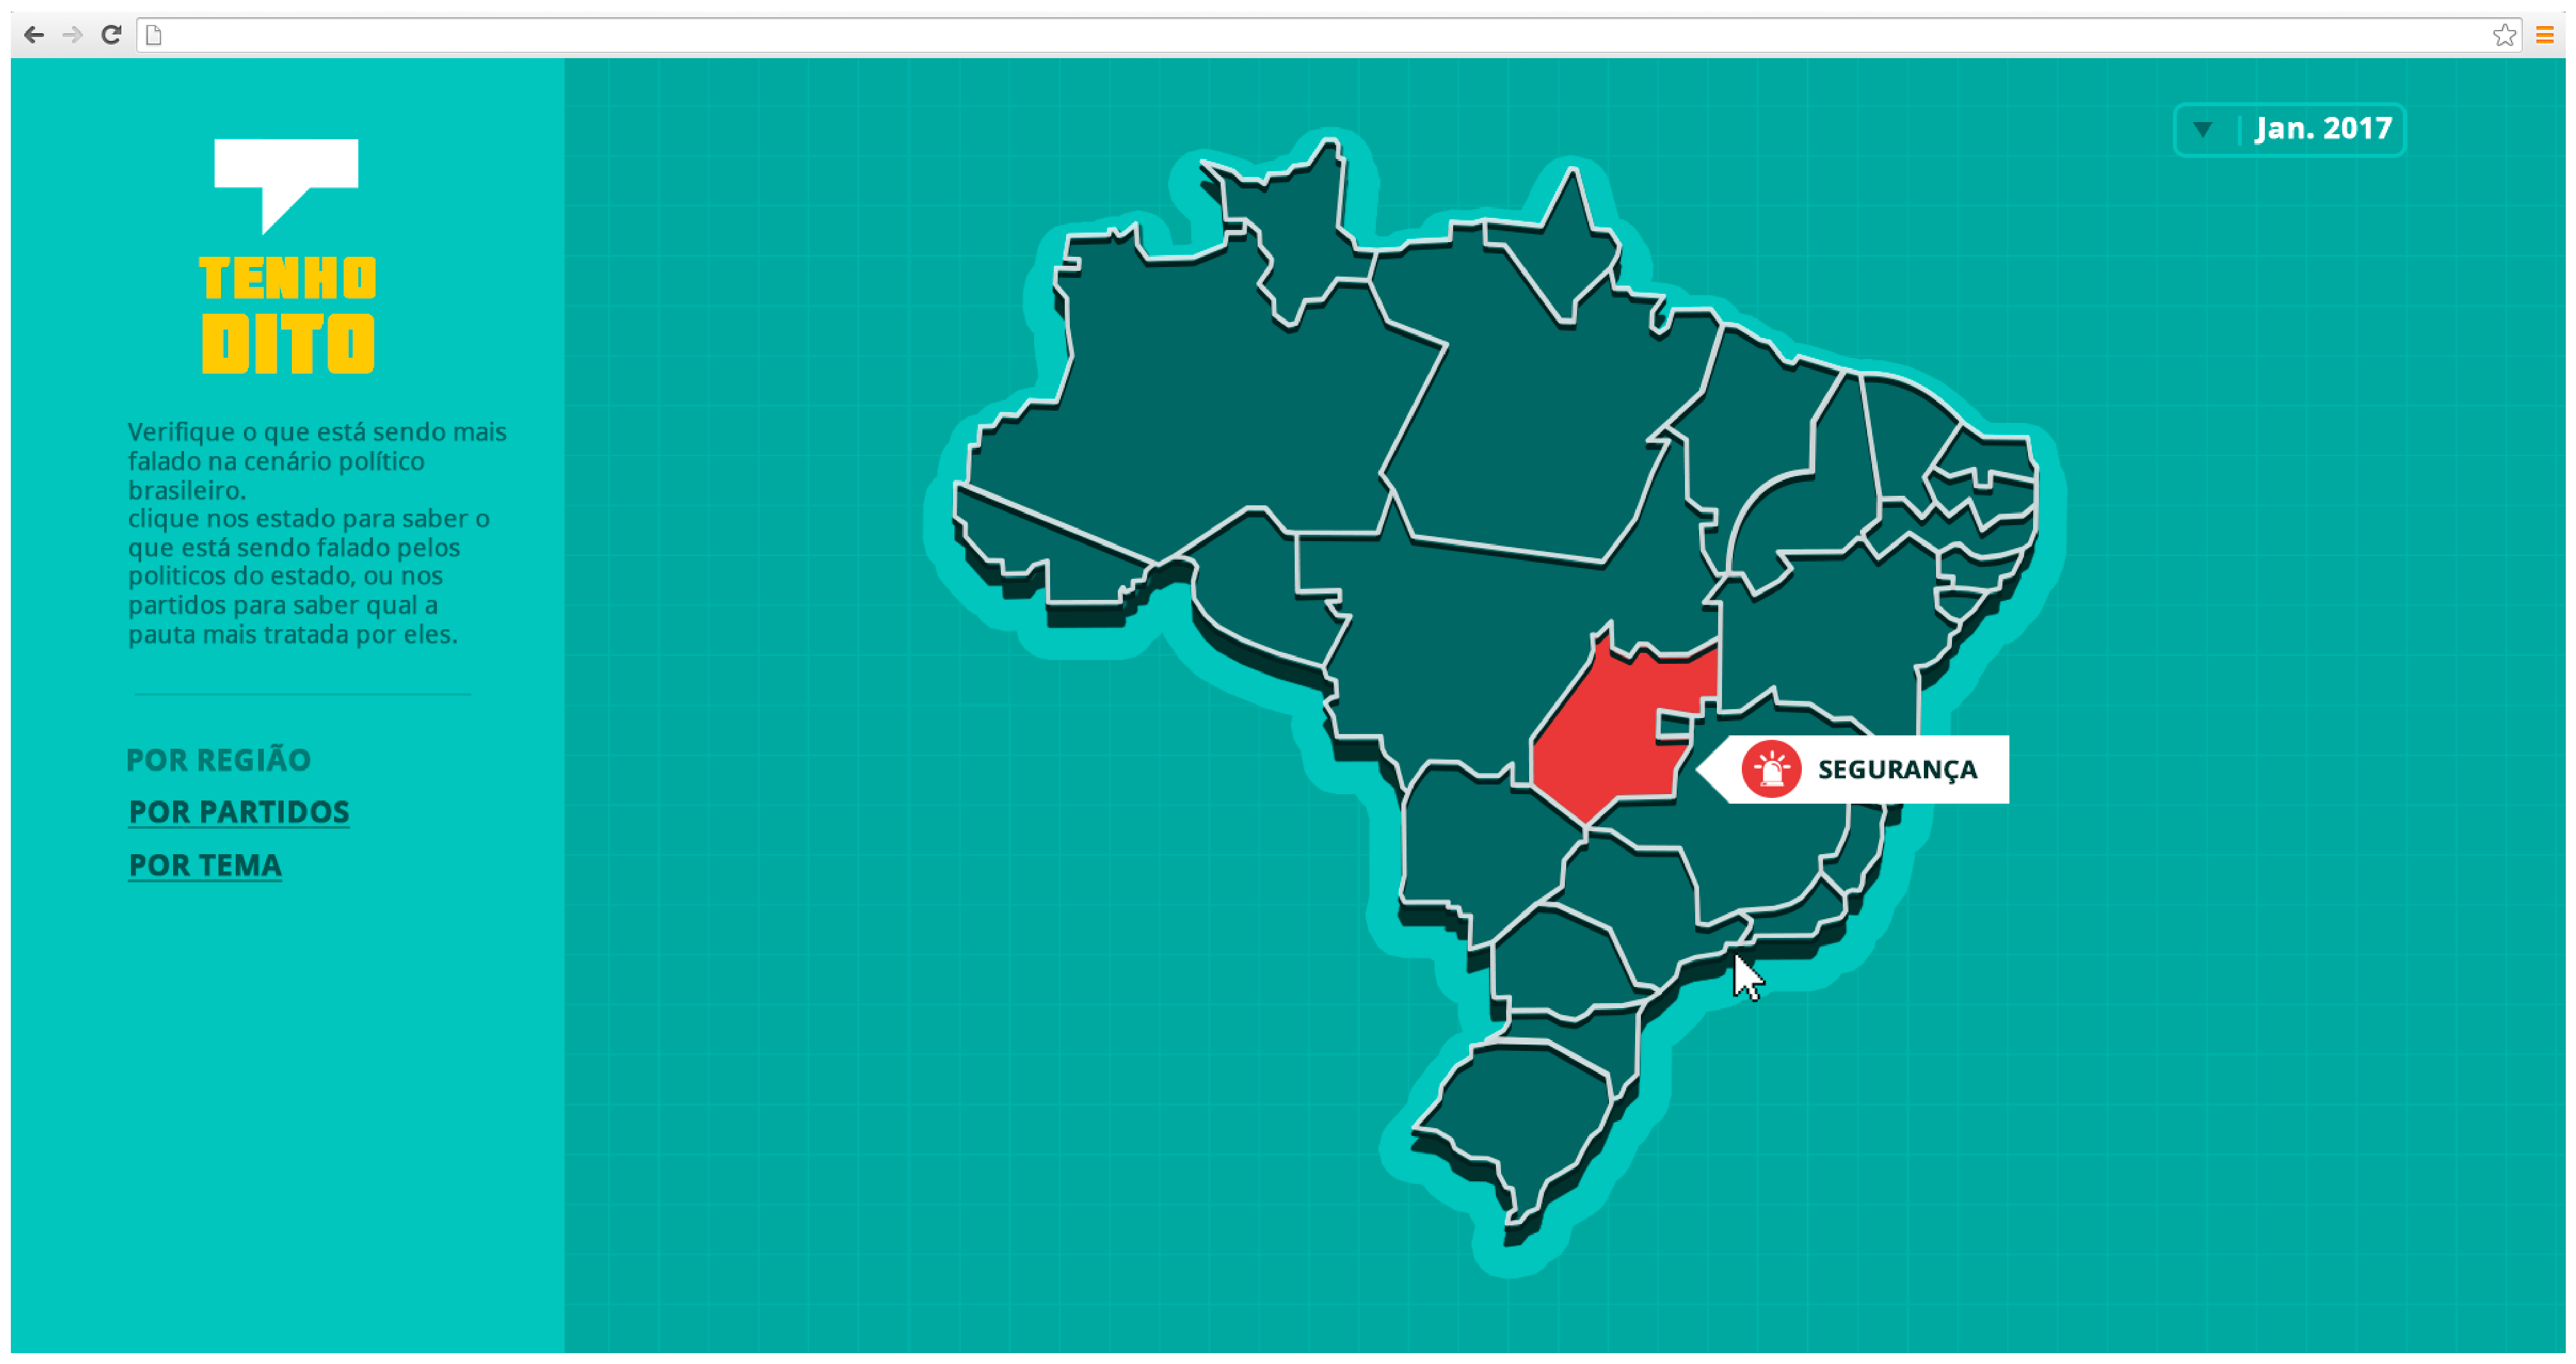
\includegraphics[scale=0.2]{figuras/tenhodito1.eps}
  \caption{Tela inicial do Tenho Dito - Visualização por região}
  \label{tenhodito1}
\end{figure}

Seguindo a abordagem por temas, ao clicar em um estado, o usuário é direcionado a outra página (figura \ref{tenhodito2}), onde encontra um gráfico de bolhas, detalhando os temas abordados pelos parlamentares do estado. Quanto maior a bolha, mais o tema foi abordado. Além disso, também são listados todos os deputados que representam aquele estado, juntamente com sua foto, partido e o tema predominante em seus discursos e proposições. Ainda não foram definidas as interações com o gráfico de bolhas.

\begin{figure}[h]
  \centering
  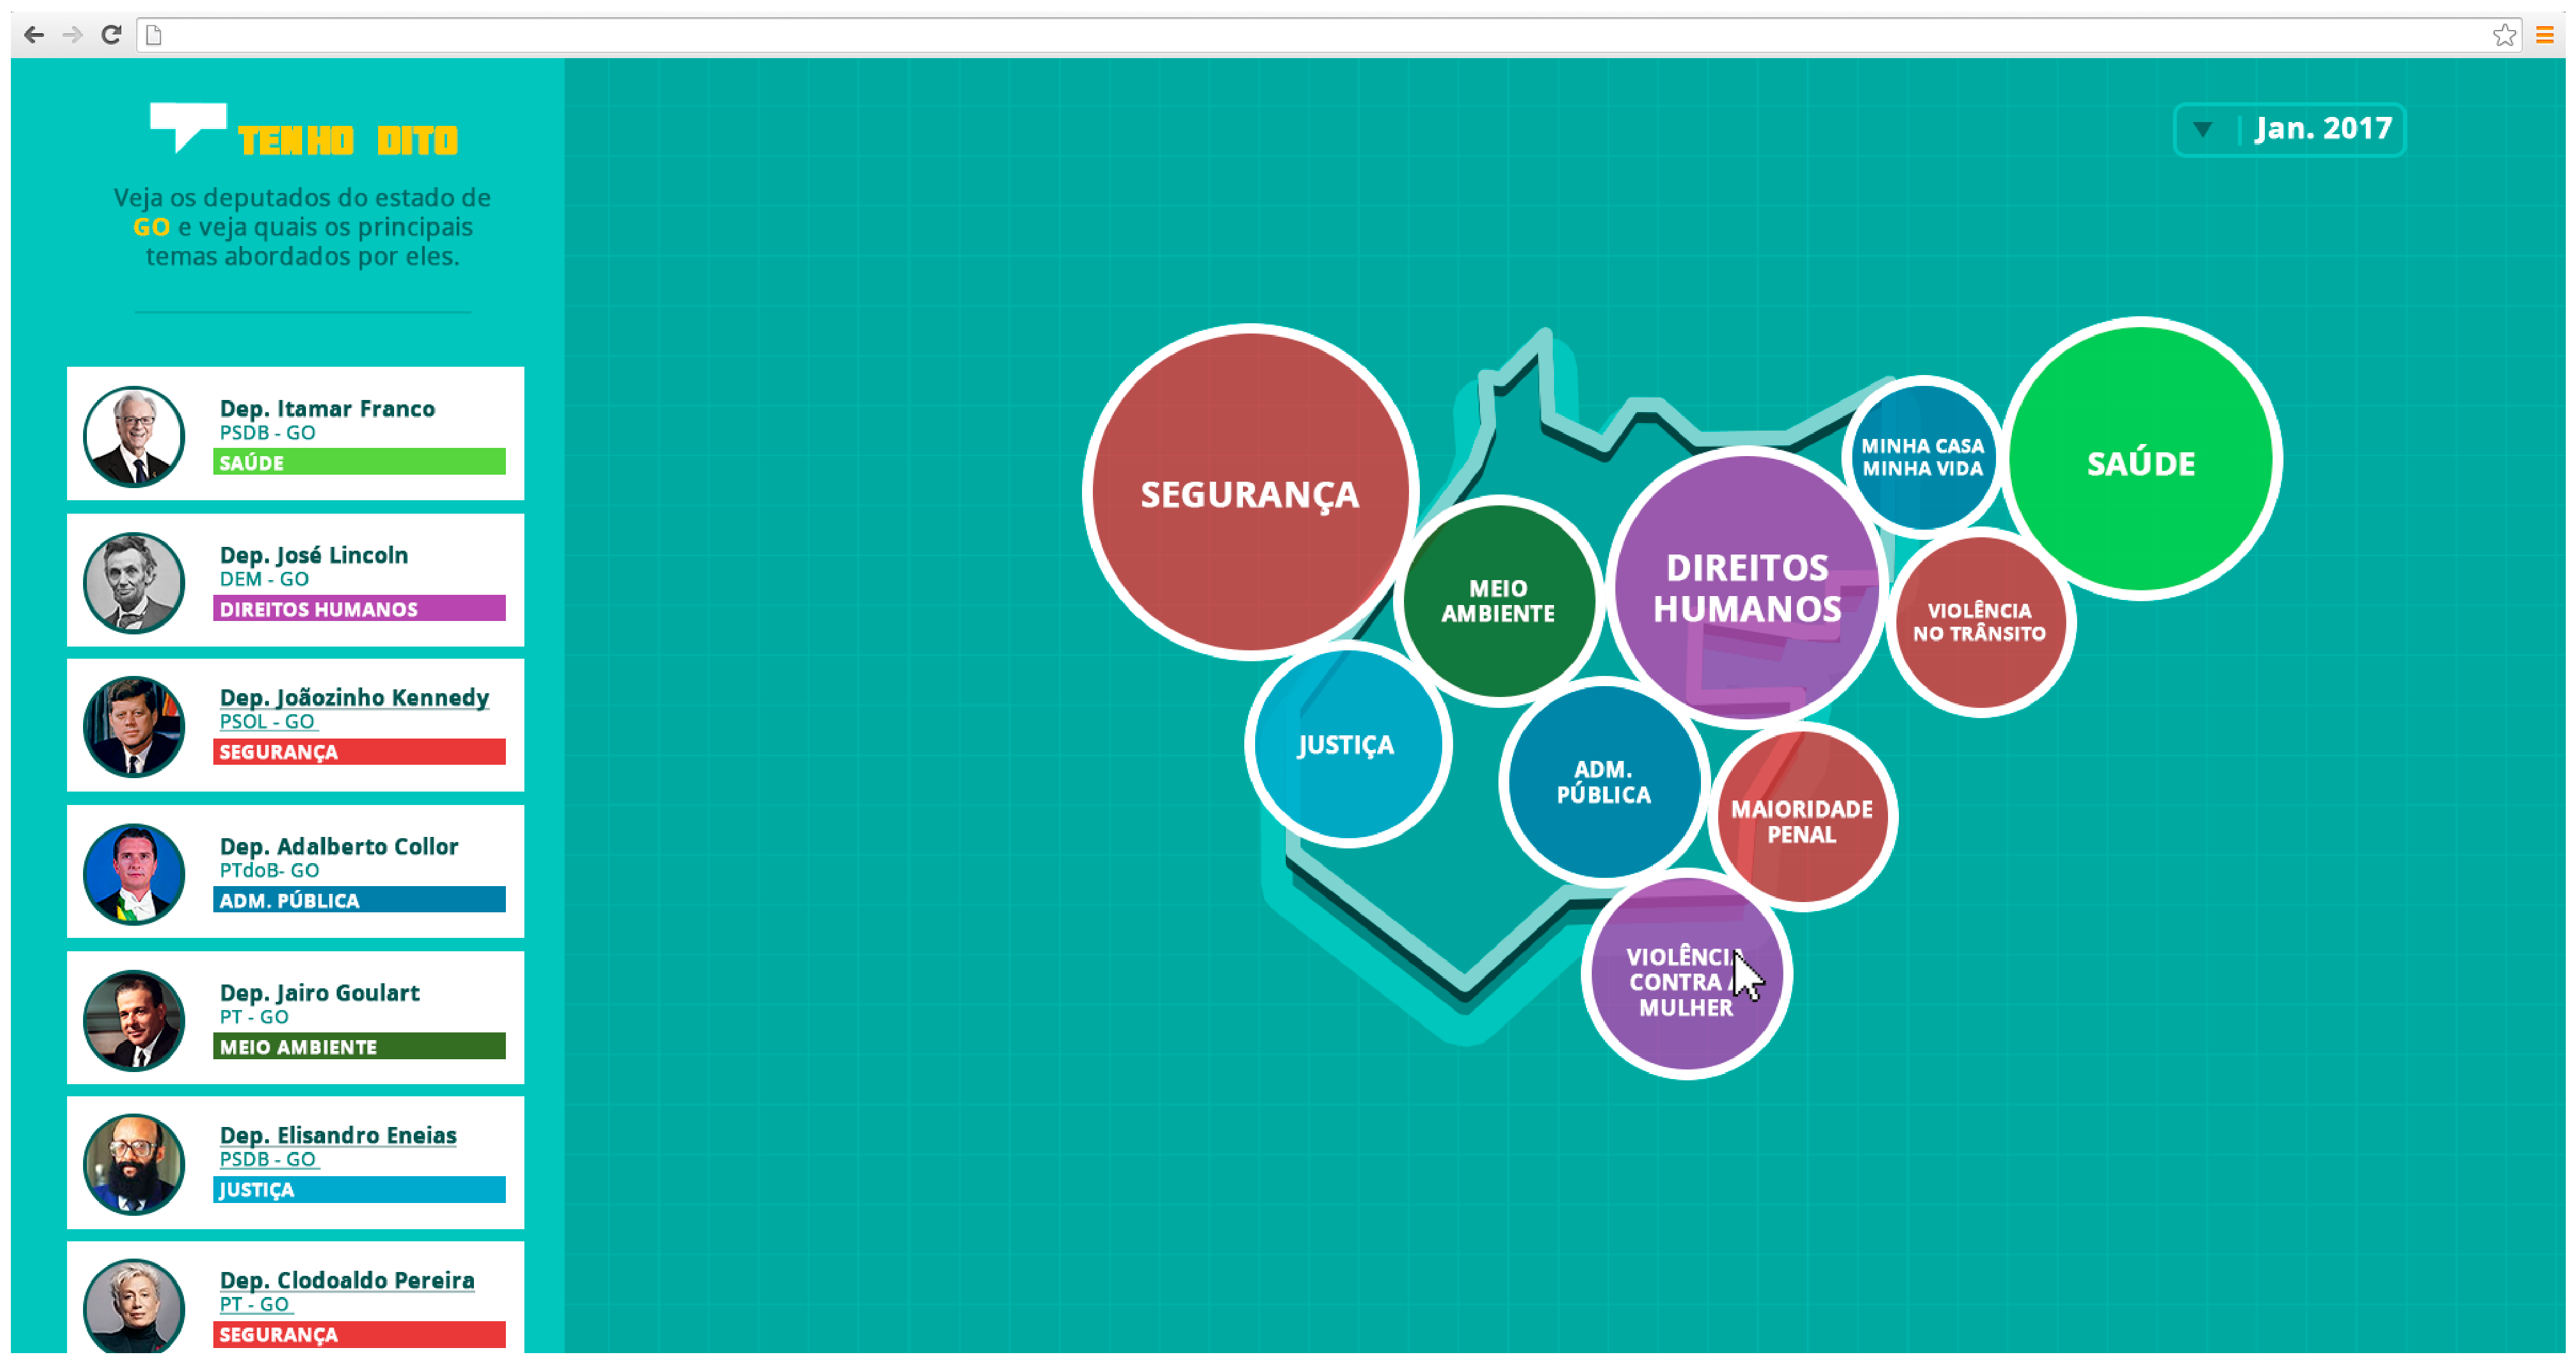
\includegraphics[scale=0.2]{figuras/tenhodito2.eps}
  \caption{Visualização detalhada dos temas, por região}
  \label{tenhodito2}
\end{figure}

O usuário também poderá selecionar um deputado específico e visualizar o seu perfil. Na tela de perfil do deputado (figura \ref{tenhodito3}), são exibidas as informações do deputado e também a quantidade de proposições e discursos analisados. Logo abaixo, será mostrado, dinâmica e randomicamente, trechos de discursos ou proposições e sua classificação. Além disso, serão listados todos os temas e a quantidade de discursos e proposições (por meio de gráfico de barras), com o objetivo de realizar uma comparação entre o que é mais dito pelo deputado e o que é mais proposto.

\begin{figure}[h]
  \centering
  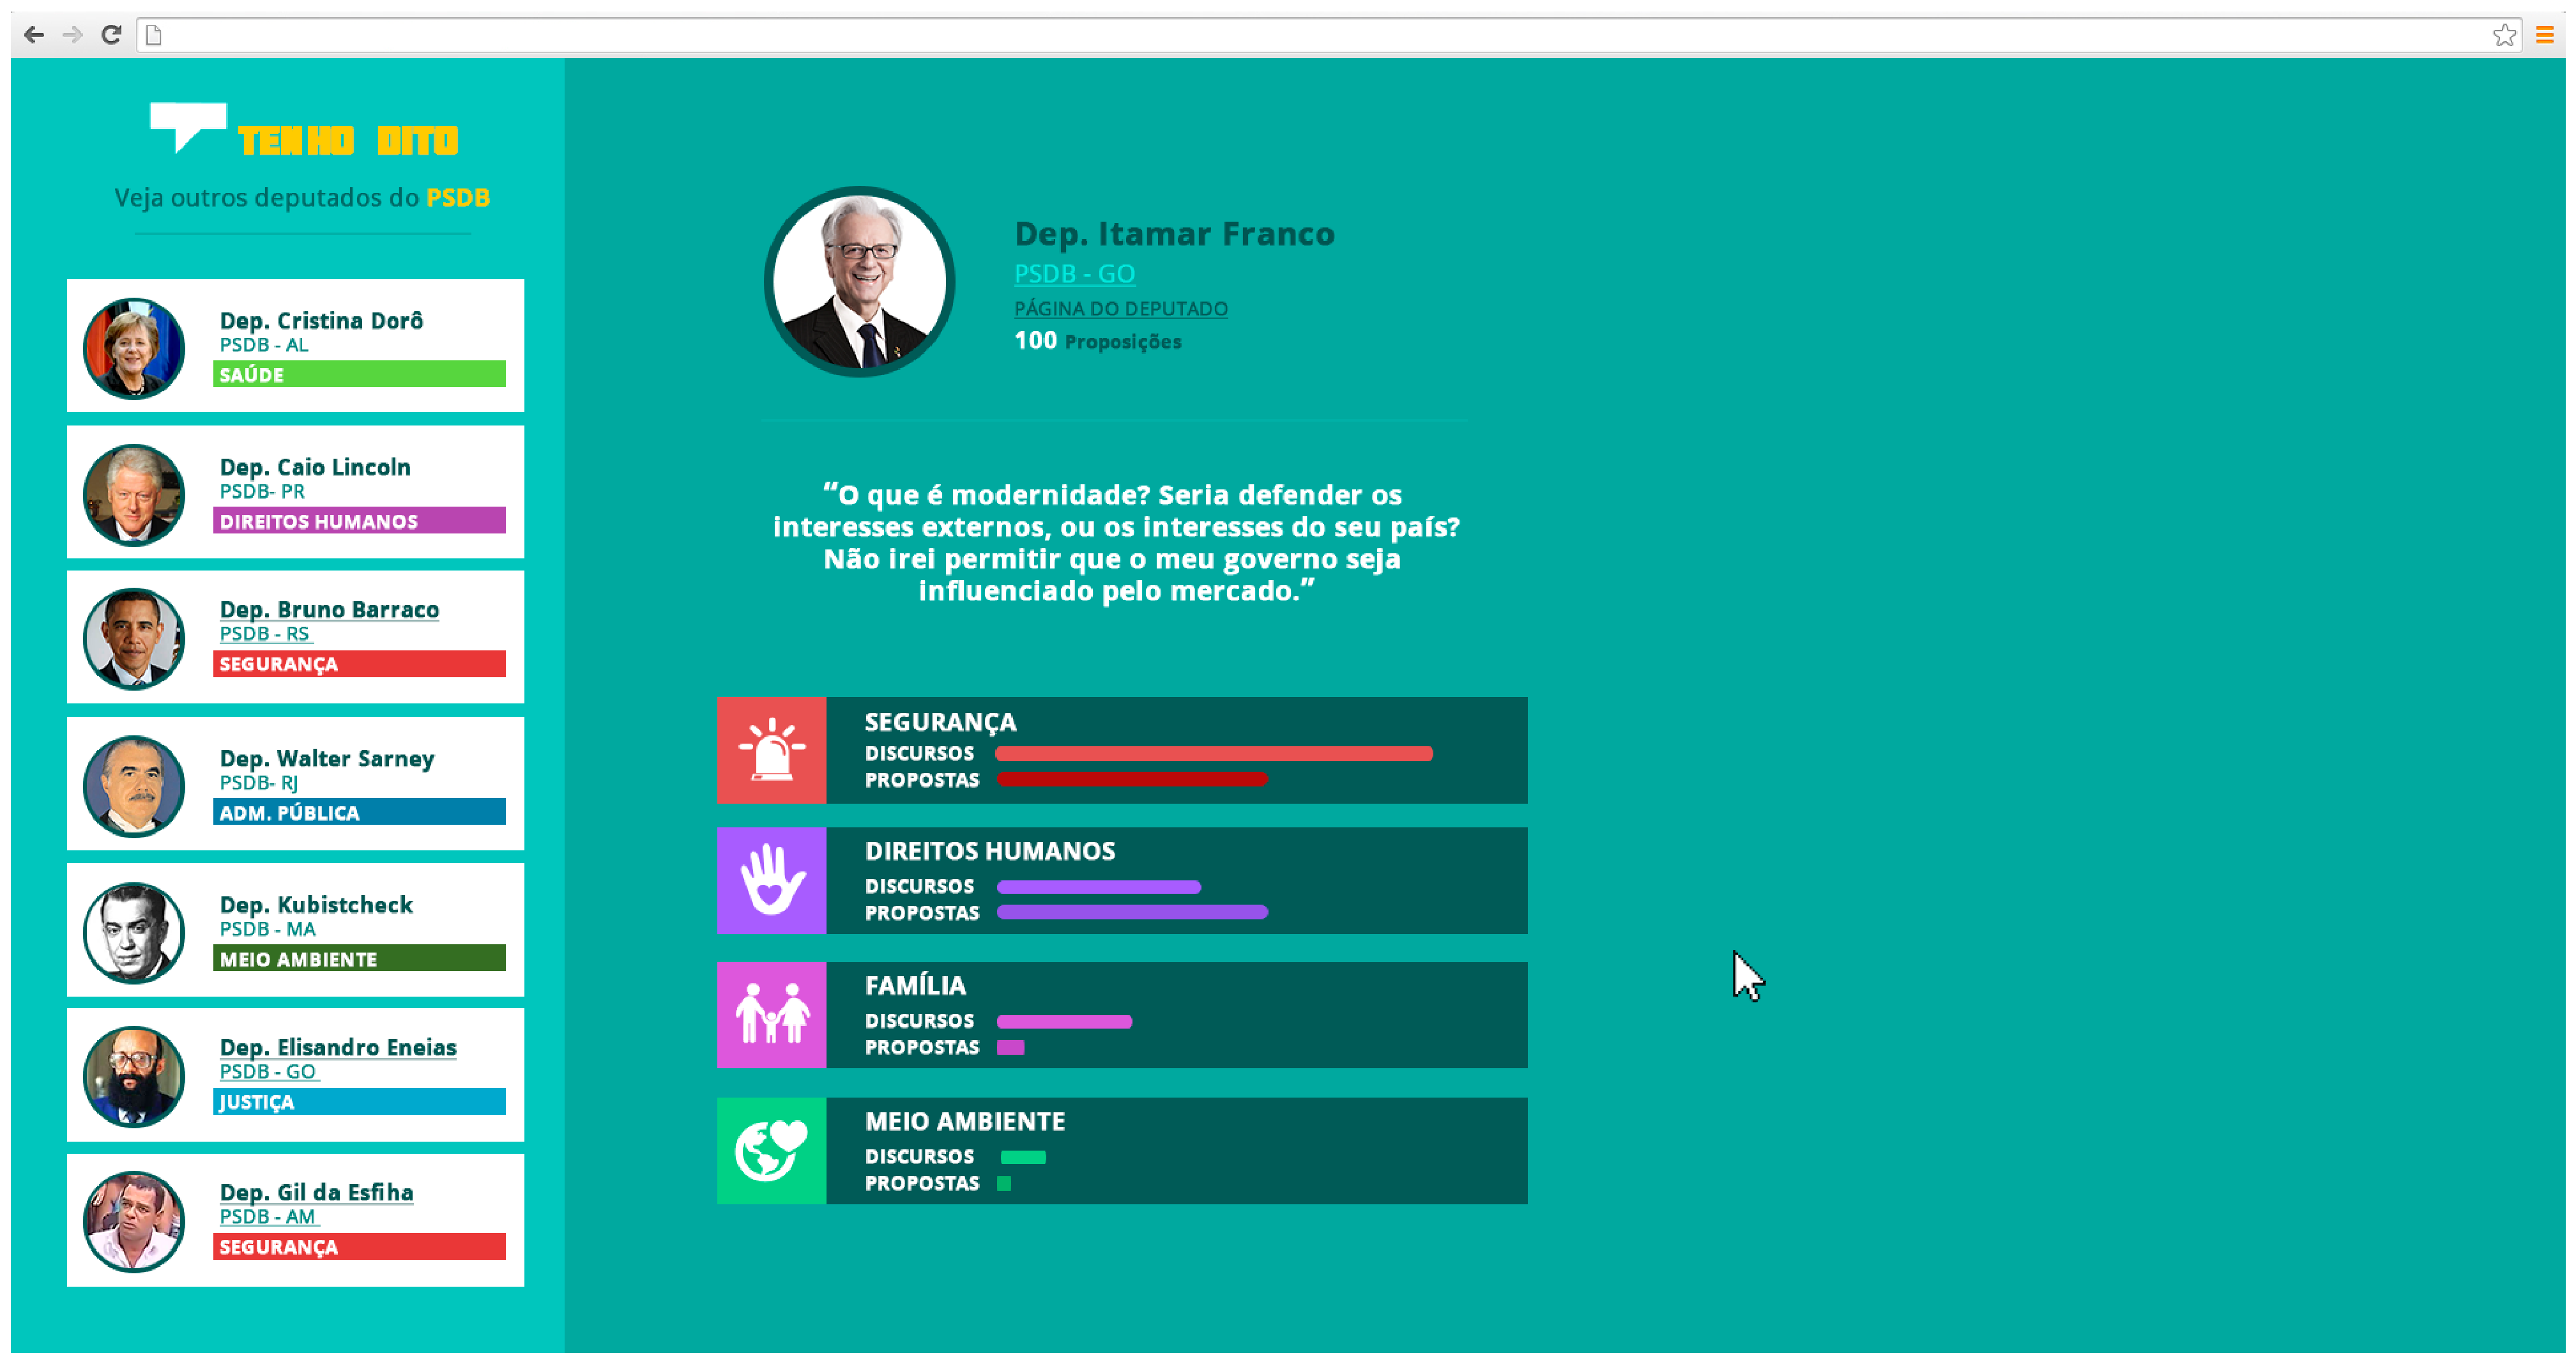
\includegraphics[scale=0.2]{figuras/tenhodito3.eps}
  \caption{Página de perfil do deputado}
  \label{tenhodito3}
\end{figure}

Quando o usuário clicar na opção de visualização por partidos, será exibida uma lista com os atuais partidos com representação na Câmara dos Deputados (figura \ref{tenhodito4}). O sitema possibilitará três tipos de ordenação: por tamanho (quantidade de deputados por partido), por ordem alfabética ou por tema. Nessa tela, também serão exibidos os temas mais abordados pelos partidos, através dos seus membros. Caso o partido tenho mais deputados cujo tema mais abordado em seus discursos e proposições é ``segurança'', por exemplo, o tema atribuído ao partido será ``segurança''.

\begin{figure}[h]
  \centering
  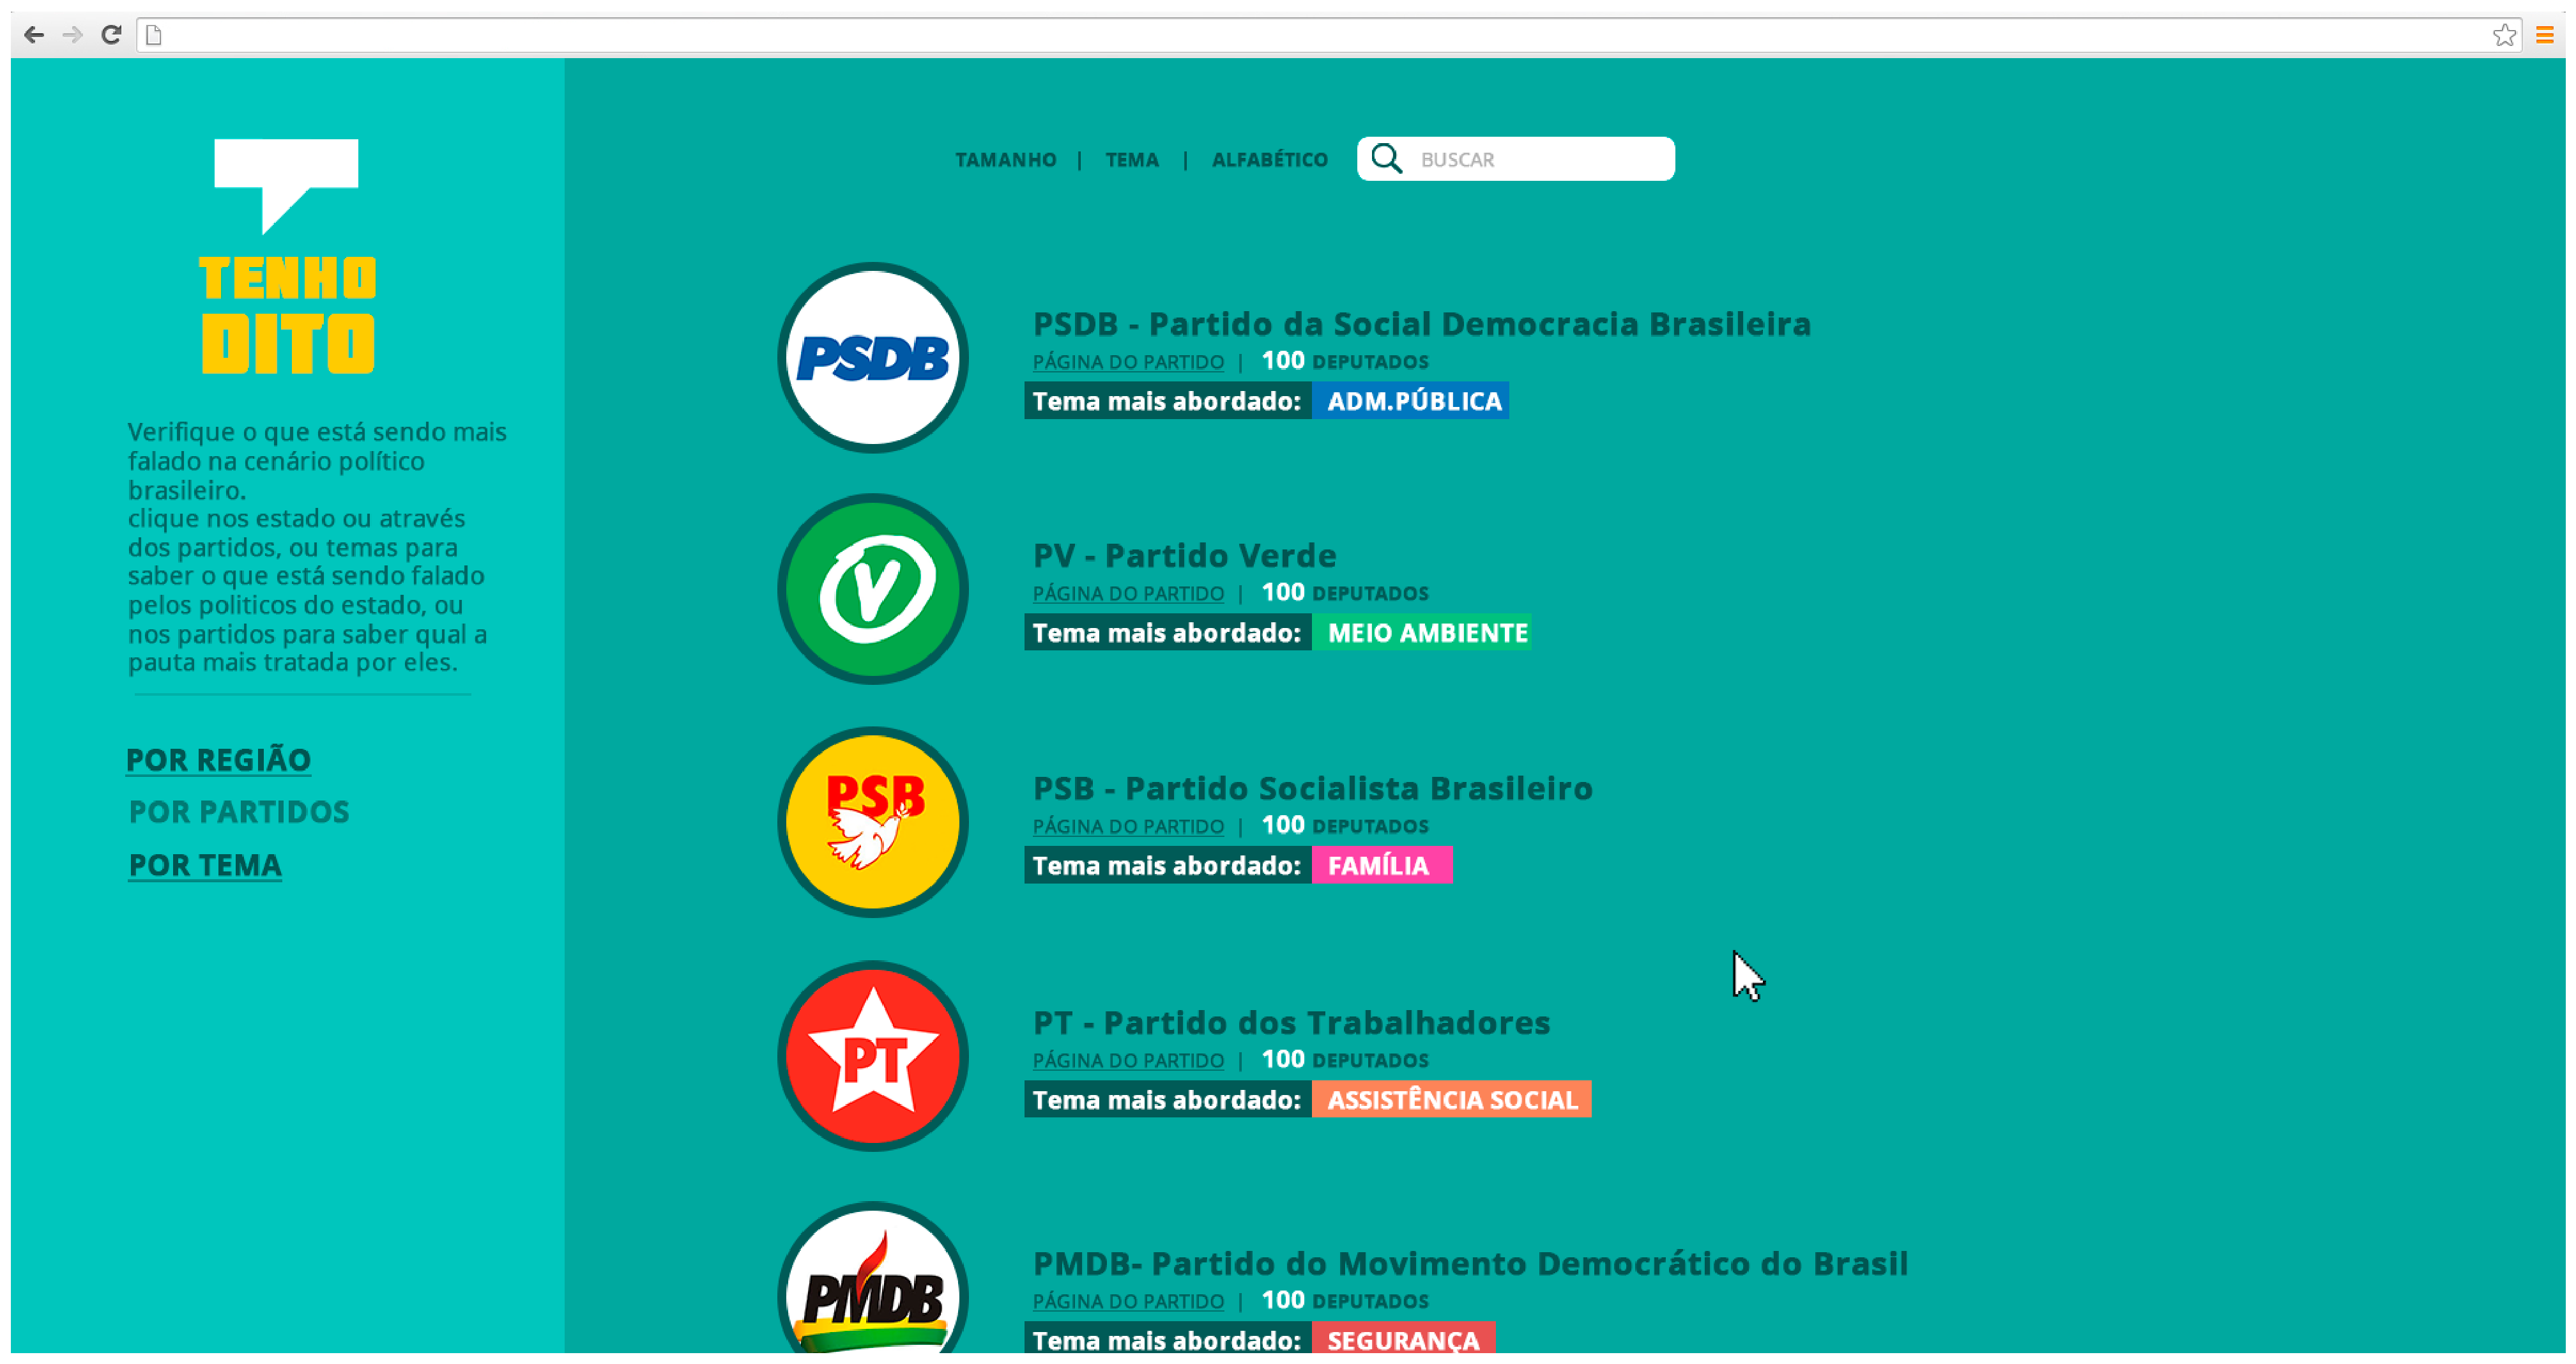
\includegraphics[scale=0.2]{figuras/tenhodito4.eps}
  \caption{Listagem dos partidos com representação na Câmara dos Deputados}
  \label{tenhodito4}
\end{figure}

O usuário poderá, assim como na abordagem por estado, escolher um partido para detalhar os temas abordados e, da mesma forma, é exibido um gráfico de bolhas com os temas abordados pelos deputados desse partido. Ao lado são mostrados todos os deputados do partido, independente do seu estado, ao clicar em algum deles o usuário é direcionado à pagina de perfil dele.

\begin{figure}[h]
  \centering
  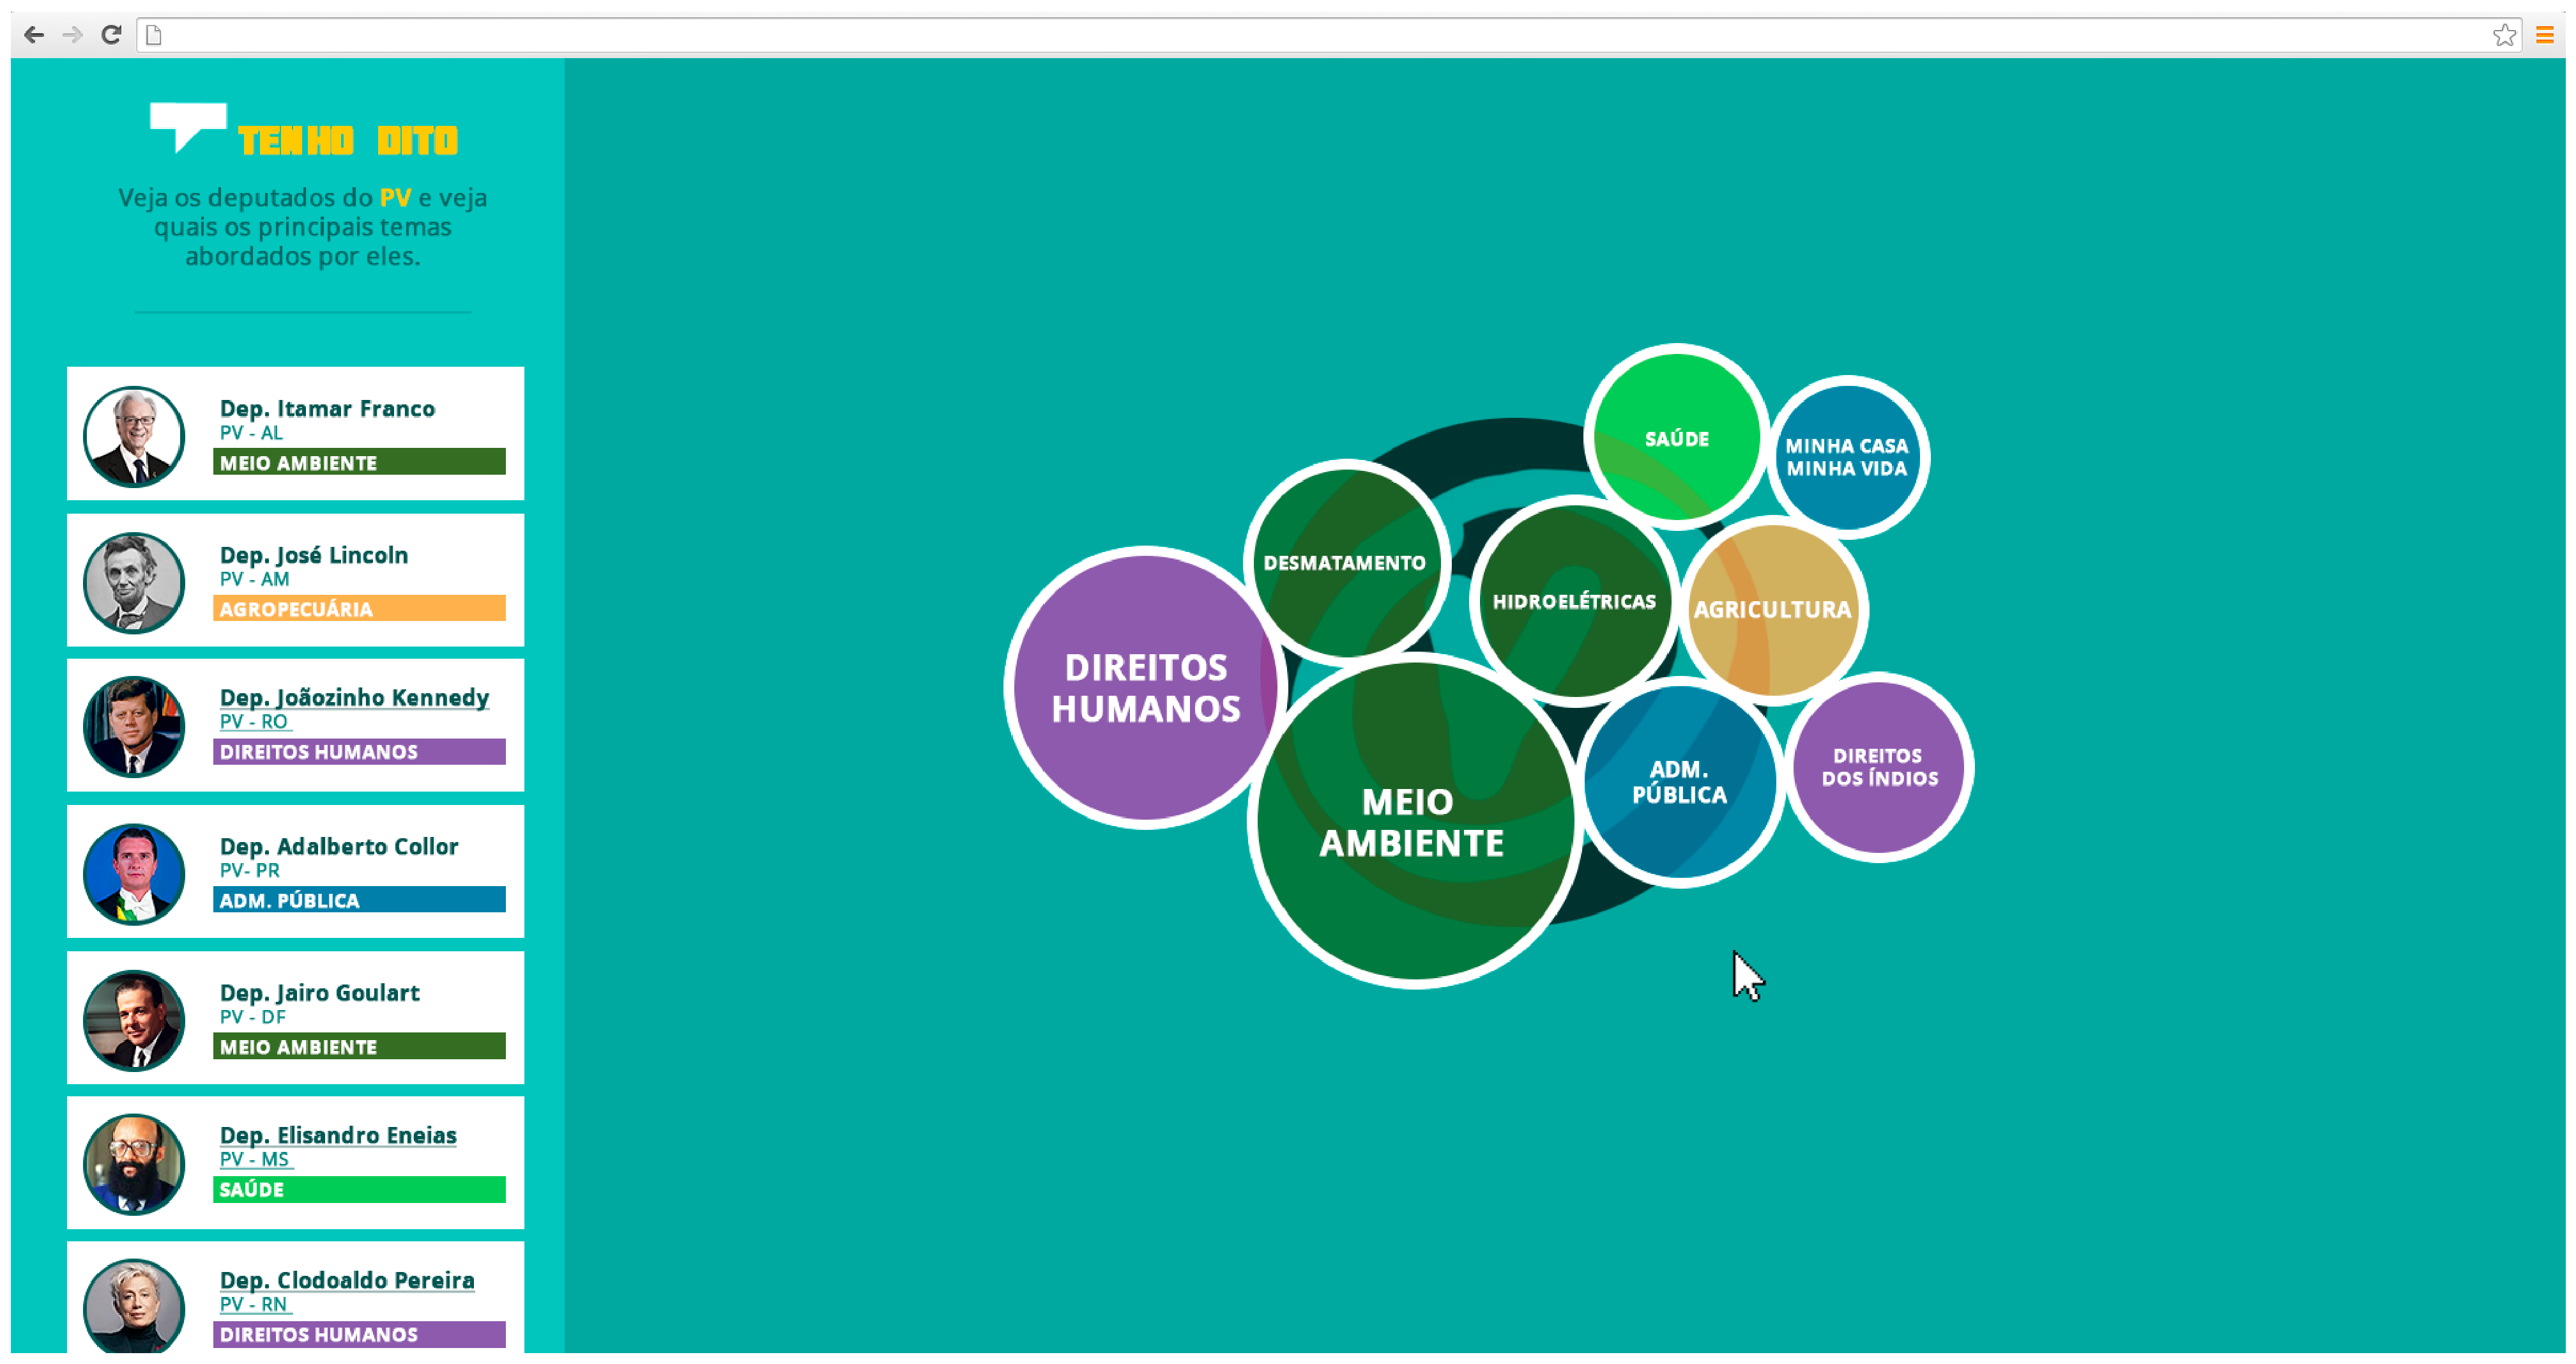
\includegraphics[scale=0.2]{figuras/tenhodito5.eps}
  \caption{Visualização detalhada dos temas, por partido}
  \label{tenhodito5}
\end{figure}

\chapter{\textit{Webservice} da Câmara dos Deputados}
\label{estrutura-webservice}

O \textit{webservice} atual (\textit{SOAP}) possui um total de 28 \textit{endpoints}, onde 5 são relacionados aos deputados, 9 aos órgãos, 9 às proposições e 5 às sessões e reuniões. A seguir descrevemos os \textit{endpoints} utilizados.

Os \textit{endpoints} que fornecem dados de deputados são:
\begin{itemize}
    \item \textbf{ObterDeputados:} retorna os deputados em exercício na Câmara dos Deputados
    \item \textbf{ObterDetalhesDeputado:} retorna detalhes dos deputados com histórico de participação em comissões, períodos de exercício, filiações partidárias e lideranças.
    \item \textbf{ObterLideresBancadas:} retorna os deputados líderes e vice-líderes em exercício das bancadas dos partidos
    \item \textbf{ObterPartidosCD:} retorna os partidos com representação na Câmara dos Deputados
    \item \textbf{ObterPartidosBlocoCD:} retorna os blocos parlamentares na Câmara dos Deputados.
\end{itemize}

Os \textit{endpoints} que fornecem dados de órgãos legislativos são:

\begin{itemize}
    \item \textbf{ListarCargosOrgaosLegislativosCD:} retorna a lista dos tipos de cargo para os órgãos legislativos da Câmara dos Deputados (ex: presidente, primeiro-secretário, etc)
    \item \textbf{ListarTiposOrgaos:} retorna a lista dos tipos de órgãos que participam do processo legislativo na Câmara dos Deputados
    \item \textbf{ObterAndamento:} retorna o andamento de uma proposição pelos órgãos internos da Câmara a partir de uma data específica
    \item \textbf{ObterEmendasSubstitutivoRedacaoFinal:} retorna as emendas, substitutivos e redações finais de uma determinada proposição
    \item \textbf{ObterIntegraComissoesRelator:} retorna os dados de relatores e pareces, e o link para a íntegra de uma determinada proposição
    \item \textbf{ObterMembrosOrgao:} retorna os parlamentares membros de uma determinada comissão
    \item \textbf{ObterOrgaos:} retorna a lista de órgãos legislativos da Câmara dos Deputados (comissões, Mesa Diretora, conselhos, etc.)
    \item \textbf{ObterPauta:} retorna as pautas das reuniões de comissões e das sessões plenárias realizadas em um determinado período
    \item \textbf{ObterRegimeTramitacaoDespacho:} retorna os dados do último despacho da proposição
\end{itemize}

Os \textit{endpoints} que fornecem dados de proposições são:

\begin{itemize}
    \item \textbf{ListarProposicoes:} retorna a lista de proposições que satisfaçam os critérios estabelecidos
    \item \textbf{ListarSiglasTipoProposicao:} retorna a lista de siglas de proposições
    \item \textbf{ListarSituacoesProposicao:} retorna a lista de situações para proposições
    \item \textbf{ListarTiposAutores:} retorna a lista de tipos de autores das proposições
    \item \textbf{ObterProposicao:} retorna os dados de uma determinada proposição a partir do tipo, número e ano
    \item \textbf{ObterProposicaoPorID:} retorna os dados de uma determinada proposição a partir do seu ID
    \item \textbf{ObterVotacaoProposicao:} retorna os votos dos deputados a uma determinada proposição em votações ocorridas no Plenário da Câmara dos Deputados
    \item \textbf{ListarProposicoesVotadasEmPlenario:} retorna todas as proposições votadas em plenário num determinado período
    \item \textbf{listarProposicoesTramitadasNoPeriodo:} retorna uma lista de proposições movimentadas em determinado período.
\end{itemize}

Os \textit{endpoints} que fornecem dados de sessões e reuniões são:

\begin{itemize}
    \item \textbf{ListarDiscursosPlenario:} retorna a lista dos deputados que proferiam discurso no Plenário da Cãmara dos Deputados em um determinado período.
    \item \textbf{ListarPresencasDia:} retorna a lista de presença de deputado em um determinado dia.
    \item \textbf{ListarPresencasParlamentar:} retorna as presenças de um deputado em um determinado período.
    \item \textbf{ListarSituacoesReuniaoSessao:} retorna a lista de situações para as reuniões de comissão e sessões plenárias da Câmara dos Deputados
    \item \textbf{ObterInteiroTeorDiscursosPlenario:} retorna o inteiro teor do discurso proferido no Plenário.
\end{itemize}

\chapter{Treinamento Inicial dos Classificadores}
\label{conjunto-palavras}

Para realizar o treinamento inicial dos classificadores \textit{naive} Bayes, é necessário fornecer um texto inicial e a sua classificação. Esse apêndice descreve os textos usados nesse trabalho para cada classificação.

\section{Classificação de Conteúdo Útil/Não-útil}

Para a classificação de ``conteúdo útil'' e ``conteúdo não-útil'', foram utilizadas os seguintes conjuntos de palavras iniciais:

\begin{itemize}
    \item \textbf{Conteúdo não-útil:} ``agradecimento agradeço muito obrigado v.exa. digníssimo nobre deputado amigo peço registro pela ordem pedir um aparte mérito emendas votado sessão comissão protocolo regimento pronunciamento divulgação''
    \item \textbf{Conteúdo útil:} ``educação universidade estudante professor ensino escola educador saúde médicos hospitais sus remédios atendimento hospitalar tratamento leitos religião templo igreja deus bíblia fé jesus segurança polícia crime violência punição arma contrabando ditadura militar golpe 31 de março tortura censura mulher aborto feminicídio feminismo feminista maria da penha petrobras pré-sal refinamento gasolina álcool combustível petrolão corrupção ministério público agu lava-jato mensalão impeachment crime de responsabilidade agronegócio agricultura agrícolas soja lavoura rural indústria desendustrialização empregos competitividade direitos humanos minorias tortura tráfego de pessoas trabalho escravo''
\end{itemize}

\section{Classificação Temática}

Para a classificação temática, os temas escolhidos e seus respectivos conjuntos de palavras utilizados foram:

\begin{itemize}
    \item \textbf{Agropecuária:} ``agropecuária fertilizantes agronegócio abate suínos ovos cabeças bovinos frangos exportação carne animal milho ração aviária laranja safra frutos pomares laranjeiras fazenda pés produzir hectares quilos fruta  produtor orgânico consumidor toneladas  embrapa bezerros pecuária veterinária filhotes sementes agro produção água sol área degradação produtor café importação agrícola pescador alimento alimentação açúcar ibge fertilizante lavouras grão bovino soja etanol frutos rural''
    \item \textbf{Saúde:} ``saúde médico doença vírus zika pesquisa paciente estudo mosquito epidemia chikungunya tratamento procedimento tremor causa gêmeos dengue transmissão cubano bebês cirurgia cientista risco sintomas dor ultrassom dr aegypt ovário microcefalia gravidez sistema imune imunológico drogas fertilização febre diagnóstico renal sangue insuficiente insuficiência cérebro idade nascimento hipotálamo morte dna corpo cardio muscular vacina''
    \item \textbf{Esporte:} ``esporte jogo jogador clube time contrato treino mundial atleta surf futebol disputa penalidade compo estádio ataque atacante bola goleiro treinador seleção técnico campeonato gol pontuação futsal vitória perde perdedor lutador torcedor torcida rival diretor falta conquista prorrogação empate surfista assistência ufc''
    \item \textbf{Educação:} ``educação estudo ensino escola médio prova enem universidade faculdade matemática avaliação aluno curso pesquisa inep exame pública mec professor redação criança texto reforma currículo curricular campus leitura literatura desempenho formação qualidade disciplina fies superior analfabeto analfabetismo português física química geometria''
    \item \textbf{Ciência e Tecnologia:} ``ciência tecnologia novidades empresa startup smart serviço smartphone consumidor produto google aparelho samsung celular internet inteligência artificial desenvolvimento dispositivo lançamento  aplicativo inovar inovação sony conectar conectado comunicação 3g 4g 5g iphone sistema telecomunicações satélite design científico artigo computador tráfego eletrônico apple whatsapp televisão tv telefone avanço espacial''
    \item \textbf{Economia:} ``economia trabalho crédito compra banco bilhões milhões vendas contas inflação consumidor juros queda crise taxa resultado econômico gasto pagamento valor financeiro investimento dinheiro índice comércio empresa desemprego fgts limite emprego cartão varejo déficite fundo recessão recuo salário lojista tesouro fiscal inadimplente recurso dólar euro moeda bolsa endividado projeções crescimento capital ações negócios''
    \item \textbf{Política:} ``política deputado congresso pt partido estado união reforma lei legislatura legislação pec pmdb aprovar voto bancada população senado senador câmara deputado sindicato candidato candidatura mandato comissão ministério constituição eleição eleições delação judiciário votações prefeitura prefeito vereador assembleia procurador corrupção''
    \item \textbf{Meio Ambiente:} ``ambiente área água rio empresa desastres multa seca barragem furacão desmatamento floresta tropical ibama parque preservação região terra planeta poluição ambiental espécie animais plantas platações petróleo emissão gás chuva temporal sol clima temperatura estufa aquecimento global umidade terremoto planeta biodiversidade biologia mar oceano calor energia sustentável madeira reflorestamento tempestade niño florescimento hídrico climática''
    \item \textbf{Direitos Humanos:} ``direitos humanos mulher tortura violência morte justiça onu sexual vítima sexual adolescente presídio prevenção união negro branco segurança refugiado homens humanitario conflito sociedade racismo sexismo machismo machista feminismo feminista defensoria estupro jovens criança prostituição assassinato liberdade idoso inclusão social preconceito gay homossexual heterosexual lgbt lésbica bissexual travesti transexual transgênero impunidade imigrante''
    \item \textbf{Segurança:} ``segurança ataque polícia suspeito morte crime terror rebelde investigação civil federal guerra onu vítima invasão preso presídio assassinato bombardeio apreensão incidente defesa exército marinha aeronáutica prisão ameaça bomba testemunha promotor policial tragédia assalto protesto''
\end{itemize}


\chapter{Índice de Incoerência}

\newcolumntype{L}[1]{>{\raggedright\let\newline\\\arraybackslash\hspace{0pt}}m{#1}}
\newcolumntype{C}[1]{>{\centering\let\newline\\\arraybackslash\hspace{0pt}}m{#1}}


A ideia inicial do Tenho Dito foi concebida em uma \textit{hackathon}, promovida pela aceleradora de \textit{startups} Cotidiano. Para a competição, o objetivo do sistema era criar um índice que mostrasse a coerência entre o que os parlamentares diziam em seus discursos em plenário e o que propunham em seus projetos de lei. Entretanto, por motivos pessoais, o autor desse trabalho preferiu não divulgar no Tenho Dito tal índice.

O Índice de Incoerência varia de 0 a 1, onde quanto maior o número, maior é a incoerência do parlamentar. Ou seja, definimos como ``incoerente'' o parlamentar que discursa muito e propõe pouco sobre um determinado tema, por exemplo.

O valor do Índice de Incoerência \(i\) é obtido através da equação:
\begin{align}
  i = \frac{\displaystyle\sum_{t}^{T} \frac{|D_{t} - P_{t}|}{max(D_{t} , P_{t})}}{Q_{T}}
\end{align}
onde:

\begin{itemize}
  \item \(T\) são todos os temas abordados pelo parlamentar,
  \item \(D_{t}\) é a porcentagem de discursos classificados como pertencentes ao tema \(t\),
  \item \(P_{t}\) é a porcentagem de proposições classificadas como pertencentes ao tema \(t\),
  \item \(max(D_{t} , P_{t})\) é o maior valor entre \(D_{t}\) e \(P_{t}\),
  \item \(Q_{T}\) é a quantidade total de temas abordados pelo parlamentar.
\end{itemize}

A tabela mostra o Índice de Incoerência obtido para cada deputado, levando em consideração os dados utilizados nesse trabalho.

\begin{longtable}{|L{4cm}|C{2cm}|C{1cm}|C{2cm}|C{1cm}|C{2cm}|}
\hline
\multicolumn{1}{|C{4cm}|}{Parlamentar} & \multicolumn{1}{C{2cm}|}{Partido} & \multicolumn{1}{C{1cm}|}{UF} & \multicolumn{1}{C{2cm}|}{Discursos} & \multicolumn{1}{C{2cm}|}{Proposições} & \multicolumn{1}{C{2cm}|}{Índice de Incoerência} \\ \hline
ADILTON SACHETTI & PSB & MT & 0 & 0 & 0 \\ \hline
ALBERTO FILHO & PMDB & MA & 0 & 0 & 0 \\ \hline
ANDRÉ DE PAULA & PSD & PE & 0 & 0 & 0 \\ \hline
ANÍBAL GOMES & PMDB & CE & 0 & 0 & 0 \\ \hline
ARIOSTO HOLANDA & PDT & CE & 0 & 0 & 0 \\ \hline
AROLDE DE OLIVEIRA & PSC & RJ & 0 & 0 & 0 \\ \hline
ARTHUR LIRA & PP & AL & 0 & 0 & 0 \\ \hline
ASSIS MELO & PCdoB & RS & 0 & 0 & 0 \\ \hline
CESAR SOUZA & PSD & SC & 0 & 0 & 0 \\ \hline
CÉSAR MESSIAS & PSB & AC & 0 & 0 & 0 \\ \hline
DEJORGE PATRÍCIO & PRB & RJ & 0 & 0 & 0 \\ \hline
DEOCLIDES MACEDO & PDT & MA & 0 & 0 & 0 \\ \hline
DIMAS FABIANO & PP & MG & 0 & 0 & 0 \\ \hline
EDMAR ARRUDA & PSD & PR & 0 & 0 & 0 \\ \hline
ELMAR NASCIMENTO & DEM & BA & 0 & 0 & 0 \\ \hline
GENECIAS NORONHA & SD & CE & 0 & 0 & 0 \\ \hline
GEORGE HILTON & PSB & MG & 0 & 0 & 0 \\ \hline
HERMES PARCIANELLO & PMDB & PR & 0 & 0 & 0 \\ \hline
IZAQUE SILVA & PSDB & SP & 0 & 0 & 0 \\ \hline
JAIME MARTINS & PSD & MG & 0 & 0 & 0 \\ \hline
JARBAS VASCONCELOS & PMDB & PE & 0 & 0 & 0 \\ \hline
JOSUÉ BENGTSON & PTB & PA & 0 & 0 & 0 \\ \hline
JOSÉ PRIANTE & PMDB & PA & 0 & 0 & 0 \\ \hline
JOÃO CARLOS BACELAR & PR & BA & 0 & 0 & 0 \\ \hline
JOÃO PAULO KLEINÜBING & PSD & SC & 0 & 0 & 0 \\ \hline
JÉSSICA SALES & PMDB & AC & 0 & 0 & 0 \\ \hline
LEONARDO QUINTÃO & PMDB & MG & 0 & 0 & 0 \\ \hline
LUANA COSTA & PSB & MA & 0 & 0 & 0 \\ \hline
LUCIANO BIVAR & PSL & PE & 0 & 0 & 0 \\ \hline
LUCIO VIEIRA LIMA & PMDB & BA & 0 & 0 & 0 \\ \hline
LUIS TIBÉ & PTdoB & MG & 0 & 0 & 0 \\ \hline
LUIZ FERNANDO FARIA & PP & MG & 0 & 0 & 0 \\ \hline
LUZIA FERREIRA & PPS & MG & 0 & 0 & 0 \\ \hline
MACEDO & PP & CE & 0 & 0 & 0 \\ \hline
MAGDA MOFATTO & PR & GO & 0 & 0 & 0 \\ \hline
MARCELO CASTRO & PMDB & PI & 0 & 0 & 0 \\ \hline
MARCELO DELAROLI & PR & RJ & 0 & 0 & 0 \\ \hline
MARCOS ABRÃO & PPS & GO & 0 & 0 & 0 \\ \hline
MARCOS MEDRADO & PODE & BA & 0 & 0 & 0 \\ \hline
MARINHA RAUPP & PMDB & RO & 0 & 0 & 0 \\ \hline
NELSON MEURER & PP & PR & 0 & 0 & 0 \\ \hline
NILSON PINTO & PSDB & PA & 0 & 0 & 0 \\ \hline
NILTON CAPIXABA & PTB & RO & 0 & 0 & 0 \\ \hline
NORMA AYUB & DEM & ES & 0 & 0 & 0 \\ \hline
PASTOR LUCIANO BRAGA & PRB & BA & 0 & 0 & 0 \\ \hline
PAULO ABI-ACKEL & PSDB & MG & 0 & 0 & 0 \\ \hline
PAULO FREIRE & PR & SP & 0 & 0 & 0 \\ \hline
PAULO MALUF & PP & SP & 0 & 0 & 0 \\ \hline
PEDRO CHAVES & PMDB & GO & 0 & 0 & 0 \\ \hline
POLLYANA GAMA & PPS & SP & 0 & 0 & 0 \\ \hline
REINHOLD STEPHANES & PSD & PR & 0 & 0 & 0 \\ \hline
RENATO ANDRADE & PP & MG & 0 & 0 & 0 \\ \hline
RICARDO TEOBALDO & PODE & PE & 0 & 0 & 0 \\ \hline
ROBERTO GÓES & PDT & AP & 0 & 0 & 0 \\ \hline
ROBINSON ALMEIDA & PT & BA & 0 & 0 & 0 \\ \hline
ROGÉRIO SILVA & PROS & MT & 0 & 0 & 0 \\ \hline
RUBENS OTONI & PT & GO & 0 & 0 & 0 \\ \hline
SABINO CASTELO BRANCO & PTB & AM & 0 & 0 & 0 \\ \hline
SARAIVA FELIPE & PMDB & MG & 0 & 0 & 0 \\ \hline
SERGIO ZVEITER & PMDB & RJ & 0 & 0 & 0 \\ \hline
SÉRGIO BRITO & PSD & BA & 0 & 0 & 0 \\ \hline
SÉRGIO MORAES & PTB & RS & 0 & 0 & 0 \\ \hline
TADEU ALENCAR & PSB & PE & 0 & 0 & 0 \\ \hline
TIRIRICA & PR & SP & 0 & 0 & 0 \\ \hline
TONINHO WANDSCHEER & PROS & PR & 0 & 0 & 0 \\ \hline
VAIDON OLIVEIRA & DEM & CE & 0 & 0 & 0 \\ \hline
VALADARES FILHO & PSB & SE & 0 & 0 & 0 \\ \hline
VITOR LIPPI & PSDB & SP & 0 & 0 & 0 \\ \hline
WALNEY ROCHA & PEN & RJ & 0 & 0 & 0 \\ \hline
WALTER IHOSHI & PSD & SP & 0 & 0 & 0 \\ \hline
WILSON BESERRA & PMDB & RJ & 0 & 0 & 0 \\ \hline
WLADIMIR COSTA & SD & PA & 0 & 0 & 0 \\ \hline
WOLNEY QUEIROZ & PDT & PE & 0 & 0 & 0 \\ \hline
YEDA CRUSIUS & PSDB & RS & 0 & 0 & 0 \\ \hline
ZECA DO PT & PT & MS & 0 & 0 & 0 \\ \hline
ZÉ AUGUSTO NALIN & PMDB & RJ & 0 & 0 & 0 \\ \hline
SILAS FREIRE & PODE & PI & 3 & 2 & 0.292 \\ \hline
ALBERTO FRAGA & DEM & DF & 64 & 66 & 0.474 \\ \hline
ANDRÉ AMARAL & PMDB & PB & 5 & 5 & 0.501 \\ \hline
CARLOS HENRIQUE GAGUIM & PODE & TO & 45 & 37 & 0.532 \\ \hline
HILDO ROCHA & PMDB & MA & 53 & 17 & 0.559 \\ \hline
RÔMULO GOUVEIA & PSD & PB & 24 & 102 & 0.587 \\ \hline
CREUZA PEREIRA & PSB & PE & 6 & 1 & 0.592 \\ \hline
CARLOS BEZERRA & PMDB & MT & 15 & 69 & 0.604 \\ \hline
FLAVINHO & PSB & SP & 9 & 26 & 0.625 \\ \hline
ROSANGELA GOMES & PRB & RJ & 8 & 2 & 0.626 \\ \hline
CABO DACIOLO & PTdoB & RJ & 7 & 12 & 0.632 \\ \hline
EDUARDO BOLSONARO & PSC & SP & 8 & 6 & 0.644 \\ \hline
MARCELO ARO & PHS & MG & 4 & 2 & 0.663 \\ \hline
NILTO TATTO & PT & SP & 17 & 10 & 0.681 \\ \hline
VITOR VALIM & PMDB & CE & 29 & 11 & 0.682 \\ \hline
AUGUSTO CARVALHO & SD & DF & 20 & 17 & 0.69 \\ \hline
VALDIR COLATTO & PMDB & SC & 35 & 9 & 0.691 \\ \hline
FRANCISCO FLORIANO & DEM & RJ & 11 & 40 & 0.692 \\ \hline
HELDER SALOMÃO & PT & ES & 5 & 8 & 0.694 \\ \hline
MIRO TEIXEIRA & REDE & RJ & 15 & 4 & 0.7 \\ \hline
MOISÉS DINIZ & PCdoB & AC & 1 & 4 & 0.704 \\ \hline
AFONSO HAMM & PP & RS & 8 & 8 & 0.706 \\ \hline
ALFREDO NASCIMENTO & PR & AM & 13 & 16 & 0.712 \\ \hline
PROFESSOR VICTÓRIO GALLI & PSC & MT & 10 & 16 & 0.724 \\ \hline
JULIO LOPES & PP & RJ & 6 & 12 & 0.727 \\ \hline
LUIZ CARLOS HAULY & PSDB & PR & 43 & 10 & 0.727 \\ \hline
CARLOS MANATO & SD & ES & 23 & 11 & 0.733 \\ \hline
ZECA CAVALCANTI & PTB & PE & 1 & 1 & 0.733 \\ \hline
AFONSO MOTTA & PDT & RS & 15 & 7 & 0.74 \\ \hline
DELEGADO EDSON MOREIRA & PR & MG & 61 & 6 & 0.742 \\ \hline
JOÃO PAULO PAPA & PSDB & SP & 1 & 4 & 0.75 \\ \hline
ROBERTO FREIRE & PPS & SP & 2 & 1 & 0.75 \\ \hline
TAKAYAMA & PSC & PR & 1 & 2 & 0.75 \\ \hline
ZÉ SILVA & SD & MG & 9 & 3 & 0.75 \\ \hline
LAURA CARNEIRO & PMDB & RJ & 19 & 37 & 0.754 \\ \hline
TENENTE LÚCIO & PSB & MG & 5 & 9 & 0.755 \\ \hline
SHÉRIDAN & PSDB & RR & 2 & 2 & 0.756 \\ \hline
LUCIANA SANTOS & PCdoB & PE & 2 & 3 & 0.757 \\ \hline
PROFESSORA DORINHA SEABRA REZENDE & DEM & TO & 3 & 5 & 0.76 \\ \hline
ROBERTO ALVES & PRB & SP & 14 & 6 & 0.76 \\ \hline
CAPITÃO AUGUSTO & PR & SP & 26 & 5 & 0.768 \\ \hline
CABO SABINO & PR & CE & 26 & 56 & 0.772 \\ \hline
LAUDIVIO CARVALHO & SD & MG & 7 & 14 & 0.775 \\ \hline
CARMEN ZANOTTO & PPS & SC & 37 & 7 & 0.78 \\ \hline
CHICO D'ANGELO & PT & RJ & 7 & 9 & 0.786 \\ \hline
ELIZIANE GAMA & PPS & MA & 7 & 2 & 0.786 \\ \hline
IRACEMA PORTELLA & PP & PI & 17 & 6 & 0.787 \\ \hline
ALCEU MOREIRA & PMDB & RS & 4 & 6 & 0.788 \\ \hline
ROCHA & PSDB & AC & 36 & 9 & 0.788 \\ \hline
BACELAR & PODE & BA & 7 & 5 & 0.79 \\ \hline
ELIZEU DIONIZIO & PSDB & MS & 6 & 8 & 0.793 \\ \hline
POMPEO DE MATTOS & PDT & RS & 27 & 9 & 0.798 \\ \hline
ALAN RICK & PRB & AC & 5 & 7 & 0.8 \\ \hline
BRUNA FURLAN & PSDB & SP & 2 & 1 & 0.8 \\ \hline
MARCO MAIA & PT & RS & 3 & 9 & 0.8 \\ \hline
VICENTINHO JÚNIOR & PR & TO & 7 & 13 & 0.801 \\ \hline
ARNALDO FARIA DE SÁ & PTB & SP & 32 & 15 & 0.802 \\ \hline
CARLOS ZARATTINI & PT & SP & 11 & 6 & 0.803 \\ \hline
RONALDO CARLETTO & PP & BA & 5 & 12 & 0.803 \\ \hline
ERIKA KOKAY & PT & DF & 88 & 14 & 0.804 \\ \hline
ROGÉRIO MARINHO & PSDB & RN & 3 & 1 & 0.806 \\ \hline
GLAUBER BRAGA & PSOL & RJ & 16 & 5 & 0.809 \\ \hline
LINCOLN PORTELA & PRB & MG & 12 & 4 & 0.81 \\ \hline
LUCIANO DUCCI & PSB & PR & 14 & 4 & 0.81 \\ \hline
RICARDO IZAR & PP & SP & 4 & 8 & 0.81 \\ \hline
PATRUS ANANIAS & PT & MG & 3 & 2 & 0.812 \\ \hline
DR. JORGE SILVA & PHS & ES & 5 & 4 & 0.815 \\ \hline
MIGUEL LOMBARDI & PR & SP & 2 & 5 & 0.815 \\ \hline
ARTHUR VIRGÍLIO BISNETO & PSDB & AM & 4 & 3 & 0.823 \\ \hline
JOÃO ARRUDA & PMDB & PR & 6 & 5 & 0.825 \\ \hline
PAULO TEIXEIRA & PT & SP & 3 & 2 & 0.828 \\ \hline
GILBERTO NASCIMENTO & PSC & SP & 19 & 3 & 0.831 \\ \hline
AELTON FREITAS & PR & MG & 2 & 1 & 0.833 \\ \hline
EDIO LOPES & PR & RR & 1 & 1 & 0.833 \\ \hline
JHC & PSB & AL & 13 & 4 & 0.834 \\ \hline
JOÃO RODRIGUES & PSD & SC & 4 & 5 & 0.834 \\ \hline
MARCOS ROGÉRIO & DEM & RO & 3 & 2 & 0.836 \\ \hline
RUBENS PEREIRA JÚNIOR & PCdoB & MA & 13 & 10 & 0.839 \\ \hline
BONIFÁCIO DE ANDRADA & PSDB & MG & 6 & 12 & 0.842 \\ \hline
MÁRCIO MARINHO & PRB & BA & 6 & 2 & 0.842 \\ \hline
ODORICO MONTEIRO & PSB & CE & 6 & 2 & 0.843 \\ \hline
VALMIR ASSUNÇÃO & PT & BA & 29 & 3 & 0.844 \\ \hline
DIEGO GARCIA & PHS & PR & 5 & 11 & 0.846 \\ \hline
RUBENS BUENO & PPS & PR & 18 & 7 & 0.846 \\ \hline
MOSES RODRIGUES & PMDB & CE & 6 & 20 & 0.847 \\ \hline
ZÉ CARLOS & PT & MA & 1 & 2 & 0.847 \\ \hline
JAIR BOLSONARO & PSC & RJ & 8 & 5 & 0.849 \\ \hline
RONALDO FONSECA & PROS & DF & 7 & 3 & 0.849 \\ \hline
ALEX MANENTE & PPS & SP & 2 & 1 & 0.85 \\ \hline
HERCULANO PASSOS & PSD & SP & 2 & 3 & 0.85 \\ \hline
JÚLIA MARINHO & PSC & PA & 3 & 3 & 0.852 \\ \hline
MARCIO ALVINO & PR & SP & 12 & 3 & 0.854 \\ \hline
PEDRO UCZAI & PT & SC & 4 & 3 & 0.854 \\ \hline
RAIMUNDO GOMES DE MATOS & PSDB & CE & 10 & 2 & 0.856 \\ \hline
LAERTE BESSA & PR & DF & 10 & 7 & 0.857 \\ \hline
IZALCI LUCAS & PSDB & DF & 6 & 4 & 0.858 \\ \hline
WEVERTON ROCHA & PDT & MA & 6 & 21 & 0.858 \\ \hline
VINICIUS CARVALHO & PRB & SP & 20 & 12 & 0.861 \\ \hline
JOÃO DERLY & REDE & RS & 5 & 22 & 0.863 \\ \hline
ARTHUR OLIVEIRA MAIA & PPS & BA & 9 & 3 & 0.866 \\ \hline
SUBTENENTE GONZAGA & PDT & MG & 3 & 6 & 0.868 \\ \hline
SÓSTENES CAVALCANTE & DEM & RJ & 15 & 12 & 0.869 \\ \hline
RAFAEL MOTTA & PSB & RN & 3 & 9 & 0.871 \\ \hline
MARCUS PESTANA & PSDB & MG & 14 & 3 & 0.874 \\ \hline
NILSON LEITÃO & PSDB & MT & 3 & 4 & 0.874 \\ \hline
KEIKO OTA & PSB & SP & 5 & 2 & 0.876 \\ \hline
CELSO PANSERA & PMDB & RJ & 2 & 4 & 0.877 \\ \hline
GEOVANIA DE SÁ & PSDB & SC & 7 & 4 & 0.877 \\ \hline
VICENTE CANDIDO & PT & SP & 1 & 2 & 0.878 \\ \hline
ALEXANDRE BALDY & PODE & GO & 6 & 1 & 0.881 \\ \hline
MAJOR OLIMPIO & SD & SP & 23 & 4 & 0.881 \\ \hline
CARLOS GOMES & PRB & RS & 4 & 2 & 0.883 \\ \hline
SEVERINO NINHO & PSB & PE & 17 & 3 & 0.884 \\ \hline
ANTONIO BULHÕES & PRB & SP & 13 & 6 & 0.885 \\ \hline
ROBERTO DE LUCENA & PV & SP & 20 & 6 & 0.888 \\ \hline
DANILO CABRAL & PSB & PE & 3 & 1 & 0.889 \\ \hline
PEPE VARGAS & PT & RS & 8 & 2 & 0.89 \\ \hline
ONYX LORENZONI & DEM & RS & 13 & 6 & 0.891 \\ \hline
MARCOS REATEGUI & PSD & AP & 7 & 3 & 0.894 \\ \hline
HEITOR SCHUCH & PSB & RS & 30 & 4 & 0.895 \\ \hline
LUCIO MOSQUINI & PMDB & RO & 2 & 4 & 0.896 \\ \hline
VALMIR PRASCIDELLI & PT & SP & 3 & 1 & 0.896 \\ \hline
DANILO FORTE & PSB & CE & 11 & 1 & 0.9 \\ \hline
WILSON FILHO & PTB & PB & 2 & 13 & 0.901 \\ \hline
DOMINGOS SÁVIO & PSDB & MG & 23 & 2 & 0.902 \\ \hline
LUIZ COUTO & PT & PB & 74 & 3 & 0.902 \\ \hline
RÔNEY NEMER & PP & DF & 2 & 3 & 0.902 \\ \hline
CAIO NARCIO & PSDB & MG & 11 & 6 & 0.903 \\ \hline
LOBBE NETO & PSDB & SP & 15 & 3 & 0.903 \\ \hline
ALESSANDRO MOLON & REDE & RJ & 4 & 2 & 0.905 \\ \hline
GOULART & PSD & SP & 3 & 26 & 0.905 \\ \hline
FELIPE MAIA & DEM & RN & 10 & 5 & 0.906 \\ \hline
DÂMINA PEREIRA & PSL & MG & 3 & 3 & 0.908 \\ \hline
GIVALDO VIEIRA & PT & ES & 24 & 2 & 0.912 \\ \hline
ESPERIDIÃO AMIN & PP & SC & 9 & 2 & 0.913 \\ \hline
CÉLIO SILVEIRA & PSDB & GO & 3 & 11 & 0.916 \\ \hline
ANTONIO CARLOS MENDES THAME & PV & SP & 2 & 4 & 0.917 \\ \hline
CHICO ALENCAR & PSOL & RJ & 36 & 2 & 0.917 \\ \hline
CONCEIÇÃO SAMPAIO & PP & AM & 2 & 2 & 0.917 \\ \hline
JOÃO CAMPOS & PRB & GO & 3 & 1 & 0.917 \\ \hline
PEDRO CUNHA LIMA & PSDB & PB & 3 & 5 & 0.917 \\ \hline
SÁGUAS MORAES & PT & MT & 18 & 2 & 0.917 \\ \hline
GERALDO RESENDE & PSDB & MS & 22 & 3 & 0.918 \\ \hline
MARA GABRILLI & PSDB & SP & 1 & 7 & 0.923 \\ \hline
FAUSTO PINATO & PP & SP & 1 & 13 & 0.924 \\ \hline
JOÃO DANIEL & PT & SE & 50 & 4 & 0.924 \\ \hline
BETO ROSADO & PP & RN & 3 & 4 & 0.927 \\ \hline
JOVAIR ARANTES & PTB & GO & 5 & 1 & 0.929 \\ \hline
BETINHO GOMES & PSDB & PE & 14 & 3 & 0.93 \\ \hline
VANDERLEI MACRIS & PSDB & SP & 10 & 2 & 0.93 \\ \hline
CACÁ LEÃO & PP & BA & 1 & 3 & 0.931 \\ \hline
TEREZA CRISTINA & PSB & MS & 2 & 3 & 0.931 \\ \hline
BENEDITA DA SILVA & PT & RJ & 24 & 2 & 0.933 \\ \hline
CABUÇU BORGES & PMDB & AP & 4 & 4 & 0.933 \\ \hline
DELEGADO WALDIR & PR & GO & 1 & 17 & 0.933 \\ \hline
JORGINHO MELLO & PR & SC & 5 & 3 & 0.933 \\ \hline
DR. SINVAL MALHEIROS & PODE & SP & 5 & 10 & 0.935 \\ \hline
VICTOR MENDES & PSD & MA & 2 & 7 & 0.936 \\ \hline
ALEXANDRE VALLE & PR & RJ & 3 & 3 & 0.937 \\ \hline
RENATO MOLLING & PP & RS & 4 & 3 & 0.937 \\ \hline
THIAGO PEIXOTO & PSD & GO & 2 & 2 & 0.937 \\ \hline
AUGUSTO COUTINHO & SD & PE & 5 & 2 & 0.938 \\ \hline
RONALDO BENEDET & PMDB & SC & 9 & 3 & 0.938 \\ \hline
ASSIS CARVALHO & PT & PI & 17 & 1 & 0.939 \\ \hline
DANIEL COELHO & PSDB & PE & 24 & 1 & 0.94 \\ \hline
PASTOR EURICO & PHS & PE & 9 & 1 & 0.941 \\ \hline
SORAYA SANTOS & PMDB & RJ & 7 & 4 & 0.941 \\ \hline
ZÉ GERALDO & PT & PA & 43 & 1 & 0.942 \\ \hline
GONZAGA PATRIOTA & PSB & PE & 38 & 2 & 0.944 \\ \hline
FÁBIO MITIDIERI & PSD & SE & 1 & 8 & 0.948 \\ \hline
JOSÉ ROCHA & PR & BA & 8 & 1 & 0.952 \\ \hline
GIOVANI CHERINI & PR & RS & 9 & 3 & 0.954 \\ \hline
NELSON PELLEGRINO & PT & BA & 3 & 1 & 0.955 \\ \hline
JOSE STÉDILE & PSB & RS & 11 & 2 & 0.958 \\ \hline
MARCUS VICENTE & PP & ES & 4 & 2 & 0.958 \\ \hline
MARIA DO ROSÁRIO & PT & RS & 21 & 1 & 0.958 \\ \hline
JÔ MORAES & PCdoB & MG & 20 & 1 & 0.959 \\ \hline
SIMÃO SESSIM & PP & RJ & 22 & 8 & 0.959 \\ \hline
LEO DE BRITO & PT & AC & 25 & 1 & 0.961 \\ \hline
GIUSEPPE VECCI & PSDB & GO & 1 & 4 & 0.964 \\ \hline
REGINALDO LOPES & PT & MG & 9 & 1 & 0.965 \\ \hline
OTAVIO LEITE & PSDB & RJ & 4 & 6 & 0.966 \\ \hline
RODRIGO PACHECO & PMDB & MG & 3 & 3 & 0.966 \\ \hline
CLEBER VERDE & PRB & MA & 6 & 15 & 0.967 \\ \hline
CRISTIANE BRASIL & PTB & RJ & 2 & 1 & 0.967 \\ \hline
ROBERTO BRITTO & PP & BA & 5 & 1 & 0.967 \\ \hline
JERÔNIMO GOERGEN & PP & RS & 1 & 15 & 0.968 \\ \hline
MARCON & PT & RS & 37 & 3 & 0.968 \\ \hline
PR. MARCO FELICIANO & PSC & SP & 18 & 2 & 0.968 \\ \hline
LUIZ SÉRGIO & PT & RJ & 11 & 1 & 0.969 \\ \hline
VICENTINHO & PT & SP & 11 & 1 & 0.971 \\ \hline
ADELMO CARNEIRO LEÃO & PT & MG & 2 & 1 & 0.972 \\ \hline
WADIH DAMOUS & PT & RJ & 2 & 6 & 0.972 \\ \hline
MARIANA CARVALHO & PSDB & RO & 5 & 22 & 0.974 \\ \hline
MARCELO MATOS & PHS & RJ & 3 & 6 & 0.975 \\ \hline
RODRIGO MARTINS & PSB & PI & 10 & 7 & 0.976 \\ \hline
JOSI NUNES & PMDB & TO & 12 & 8 & 0.979 \\ \hline
IVAN VALENTE & PSOL & SP & 37 & 2 & 0.98 \\ \hline
LUIZ LAURO FILHO & PSB & SP & 1 & 12 & 0.981 \\ \hline
SERGIO SOUZA & PMDB & PR & 7 & 1 & 0.981 \\ \hline
ANA PERUGINI & PT & SP & 2 & 6 & 0.982 \\ \hline
HENRIQUE FONTANA & PT & RS & 8 & 1 & 0.982 \\ \hline
MARIA HELENA & PSB & RR & 6 & 1 & 0.983 \\ \hline
LUIZA ERUNDINA & PSOL & SP & 7 & 1 & 0.984 \\ \hline
PAES LANDIM & PTB & PI & 28 & 2 & 0.984 \\ \hline
DANIEL VILELA & PMDB & GO & 3 & 7 & 0.985 \\ \hline
DAVIDSON MAGALHÃES & PCdoB & BA & 18 & 1 & 0.985 \\ \hline
BENJAMIN MARANHÃO & SD & PB & 10 & 1 & 0.986 \\ \hline
CHICO LOPES & PCdoB & CE & 28 & 2 & 0.986 \\ \hline
FÉLIX MENDONÇA JÚNIOR & PDT & BA & 1 & 8 & 0.986 \\ \hline
JOSÉ GUIMARÃES & PT & CE & 6 & 2 & 0.987 \\ \hline
PAULO AZI & DEM & BA & 2 & 5 & 0.987 \\ \hline
FLÁVIA MORAIS & PDT & GO & 1 & 10 & 0.989 \\ \hline
VANDER LOUBET & PT & MS & 1 & 3 & 0.989 \\ \hline
PAULO FOLETTO & PSB & ES & 16 & 1 & 0.99 \\ \hline
DANIEL ALMEIDA & PCdoB & BA & 23 & 1 & 0.992 \\ \hline
GORETE PEREIRA & PR & CE & 3 & 6 & 0.992 \\ \hline
CAETANO & PT & BA & 12 & 1 & 0.993 \\ \hline
EZEQUIEL TEIXEIRA & PODE & RJ & 2 & 7 & 0.993 \\ \hline
JEFFERSON CAMPOS & PSD & SP & 20 & 2 & 0.993 \\ \hline
ROBERTO SALES & PRB & RJ & 1 & 1 & 0.993 \\ \hline
ALIEL MACHADO & REDE & PR & 15 & 1 & 0.994 \\ \hline
COVATTI FILHO & PP & RS & 2 & 9 & 0.994 \\ \hline
STEFANO AGUIAR & PSD & MG & 11 & 1 & 0.994 \\ \hline
CELSO RUSSOMANNO & PRB & SP & 1 & 6 & 0.995 \\ \hline
CELSO MALDANER & PMDB & SC & 33 & 1 & 0.996 \\ \hline
CHRISTIANE DE SOUZA YARED & PR & PR & 1 & 7 & 0.996 \\ \hline
ARNALDO JORDY & PPS & PA & 40 & 1 & 0.998 \\ \hline
FELIPE BORNIER & PROS & RJ & 1 & 46 & 0.998 \\ \hline
JANETE CAPIBERIBE & PSB & AP & 35 & 1 & 0.998 \\ \hline
ABEL MESQUITA JR. & DEM & RR & 1 & 0 & 1 \\ \hline
ADAIL CARNEIRO & PP & CE & 1 & 5 & 1 \\ \hline
ADALBERTO CAVALCANTI & PTB & PE & 1 & 1 & 1 \\ \hline
ADELSON BARRETO & PR & SE & 1 & 0 & 1 \\ \hline
ADEMIR CAMILO & PODE & MG & 0 & 1 & 1 \\ \hline
AFONSO FLORENCE & PT & BA & 12 & 0 & 1 \\ \hline
AGUINALDO RIBEIRO & PP & PB & 1 & 0 & 1 \\ \hline
ALEX CANZIANI & PTB & PR & 4 & 0 & 1 \\ \hline
ALEXANDRE LEITE & DEM & SP & 0 & 10 & 1 \\ \hline
ALEXANDRE SERFIOTIS & PMDB & RJ & 3 & 0 & 1 \\ \hline
ALFREDO KAEFER & PSL & PR & 7 & 0 & 1 \\ \hline
ALICE PORTUGAL & PCdoB & BA & 6 & 1 & 1 \\ \hline
ALTINEU CÔRTES & PMDB & RJ & 2 & 0 & 1 \\ \hline
ALUISIO MENDES & PODE & MA & 1 & 2 & 1 \\ \hline
ANDRE MOURA & PSC & SE & 4 & 0 & 1 \\ \hline
ANDRES SANCHEZ & PT & SP & 2 & 1 & 1 \\ \hline
ANDRÉ ABDON & PP & AP & 0 & 2 & 1 \\ \hline
ANDRÉ FIGUEIREDO & PDT & CE & 0 & 1 & 1 \\ \hline
ANDRÉ FUFUCA & PP & MA & 1 & 1 & 1 \\ \hline
ANGELIM & PT & AC & 23 & 0 & 1 \\ \hline
ANTONIO BRITO & PSD & BA & 1 & 3 & 1 \\ \hline
ANTÔNIO JÁCOME & PODE & RN & 2 & 0 & 1 \\ \hline
ARLINDO CHINAGLIA & PT & SP & 1 & 0 & 1 \\ \hline
ASSIS DO COUTO & PDT & PR & 1 & 0 & 1 \\ \hline
AUREO & SD & RJ & 0 & 10 & 1 \\ \hline
BALEIA ROSSI & PMDB & SP & 4 & 1 & 1 \\ \hline
BEBETO & PSB & BA & 7 & 0 & 1 \\ \hline
BENITO GAMA & PTB & BA & 7 & 0 & 1 \\ \hline
BETO FARO & PT & PA & 1 & 0 & 1 \\ \hline
BETO MANSUR & PRB & SP & 8 & 0 & 1 \\ \hline
BETO SALAME & PP & PA & 0 & 4 & 1 \\ \hline
BILAC PINTO & PR & MG & 4 & 0 & 1 \\ \hline
BOHN GASS & PT & RS & 21 & 0 & 1 \\ \hline
BRUNNY & PR & MG & 3 & 2 & 1 \\ \hline
CAJAR NARDES & PR & RS & 0 & 3 & 1 \\ \hline
CARLOS ANDRADE & PHS & RR & 6 & 0 & 1 \\ \hline
CARLOS EDUARDO CADOCA & PDT & PE & 0 & 1 & 1 \\ \hline
CARLOS MARUN & PMDB & MS & 5 & 0 & 1 \\ \hline
CARLOS MELLES & DEM & MG & 3 & 0 & 1 \\ \hline
CARLOS SAMPAIO & PSDB & SP & 1 & 0 & 1 \\ \hline
CELSO JACOB & PMDB & RJ & 0 & 11 & 1 \\ \hline
CLAUDIO CAJADO & DEM & BA & 7 & 0 & 1 \\ \hline
CÉSAR HALUM & PRB & TO & 1 & 4 & 1 \\ \hline
CÍCERO ALMEIDA & PMDB & AL & 0 & 2 & 1 \\ \hline
DAGOBERTO NOGUEIRA & PDT & MS & 0 & 3 & 1 \\ \hline
DAMIÃO FELICIANO & PDT & PB & 2 & 2 & 1 \\ \hline
DANRLEI DE DEUS HINTERHOLZ & PSD & RS & 1 & 2 & 1 \\ \hline
DARCÍSIO PERONDI & PMDB & RS & 23 & 0 & 1 \\ \hline
DELEGADO FRANCISCHINI & SD & PR & 0 & 2 & 1 \\ \hline
DELEGADO ÉDER MAURO & PSD & PA & 8 & 0 & 1 \\ \hline
DELEY & PTB & RJ & 1 & 2 & 1 \\ \hline
DIEGO ANDRADE & PSD & MG & 0 & 6 & 1 \\ \hline
DILCEU SPERAFICO & PP & PR & 0 & 1 & 1 \\ \hline
DOMINGOS NETO & PSD & CE & 2 & 0 & 1 \\ \hline
DULCE MIRANDA & PMDB & TO & 1 & 3 & 1 \\ \hline
DÉCIO LIMA & PT & SC & 15 & 0 & 1 \\ \hline
EDMILSON RODRIGUES & PSOL & PA & 58 & 0 & 1 \\ \hline
EDUARDO BARBOSA & PSDB & MG & 0 & 11 & 1 \\ \hline
EDUARDO CURY & PSDB & SP & 4 & 0 & 1 \\ \hline
EDUARDO DA FONTE & PP & PE & 0 & 2 & 1 \\ \hline
EFRAIM FILHO & DEM & PB & 4 & 1 & 1 \\ \hline
ELCIONE BARBALHO & PMDB & PA & 0 & 1 & 1 \\ \hline
ELI CORRÊA FILHO & DEM & SP & 0 & 2 & 1 \\ \hline
ENIO VERRI & PT & PR & 5 & 0 & 1 \\ \hline
ERIVELTON SANTANA & PEN & BA & 0 & 2 & 1 \\ \hline
EROS BIONDINI & PROS & MG & 0 & 4 & 1 \\ \hline
EVAIR VIEIRA DE MELO & PV & ES & 6 & 1 & 1 \\ \hline
EVANDRO GUSSI & PV & SP & 6 & 0 & 1 \\ \hline
EVANDRO ROMAN & PSD & PR & 0 & 3 & 1 \\ \hline
EXPEDITO NETTO & PSD & RO & 4 & 0 & 1 \\ \hline
EZEQUIEL FONSECA & PP & MT & 1 & 2 & 1 \\ \hline
FABIO GARCIA & PSB & MT & 4 & 0 & 1 \\ \hline
FABIO REIS & PMDB & SE & 1 & 0 & 1 \\ \hline
FERNANDO MONTEIRO & PP & PE & 0 & 1 & 1 \\ \hline
FLAVIANO MELO & PMDB & AC & 5 & 0 & 1 \\ \hline
FRANCISCO CHAPADINHA & PODE & PA & 0 & 17 & 1 \\ \hline
FRANKLIN & PP & MG & 0 & 4 & 1 \\ \hline
FÁBIO FARIA & PSD & RN & 3 & 1 & 1 \\ \hline
FÁBIO RAMALHO & PMDB & MG & 3 & 0 & 1 \\ \hline
FÁBIO SOUSA & PSDB & GO & 6 & 4 & 1 \\ \hline
GABRIEL GUIMARÃES & PT & MG & 0 & 1 & 1 \\ \hline
GIACOBO & PR & PR & 3 & 0 & 1 \\ \hline
GIVALDO CARIMBÃO & PHS & AL & 2 & 0 & 1 \\ \hline
GUILHERME COELHO & PSDB & PE & 1 & 0 & 1 \\ \hline
GUILHERME MUSSI & PP & SP & 0 & 3 & 1 \\ \hline
HERÁCLITO FORTES & PSB & PI & 23 & 0 & 1 \\ \hline
HEULER CRUVINEL & PSD & GO & 0 & 1 & 1 \\ \hline
HIRAN GONÇALVES & PP & RR & 0 & 1 & 1 \\ \hline
HISSA ABRAHÃO & PDT & AM & 3 & 1 & 1 \\ \hline
HUGO LEAL & PSB & RJ & 1 & 2 & 1 \\ \hline
HUGO MOTTA & PMDB & PB & 1 & 1 & 1 \\ \hline
HÉLIO LEITE & DEM & PA & 2 & 1 & 1 \\ \hline
IRAJÁ ABREU & PSD & TO & 1 & 2 & 1 \\ \hline
IRMÃO LAZARO & PSC & BA & 0 & 1 & 1 \\ \hline
JANDIRA FEGHALI & PCdoB & RJ & 13 & 1 & 1 \\ \hline
JEAN WYLLYS & PSOL & RJ & 0 & 7 & 1 \\ \hline
JHONATAN DE JESUS & PRB & RR & 0 & 3 & 1 \\ \hline
JOAQUIM PASSARINHO & PSD & PA & 11 & 0 & 1 \\ \hline
JONES MARTINS & PMDB & RS & 19 & 0 & 1 \\ \hline
JONY MARCOS & PRB & SE & 3 & 0 & 1 \\ \hline
JORGE BOEIRA & PP & SC & 1 & 0 & 1 \\ \hline
JORGE CÔRTE REAL & PTB & PE & 1 & 3 & 1 \\ \hline
JORGE SOLLA & PT & BA & 14 & 1 & 1 \\ \hline
JORGE TADEU MUDALEN & DEM & SP & 2 & 0 & 1 \\ \hline
JOSÉ AIRTON CIRILO & PT & CE & 12 & 1 & 1 \\ \hline
JOSÉ CARLOS ALELUIA & DEM & BA & 3 & 0 & 1 \\ \hline
JOSÉ CARLOS ARAÚJO & PR & BA & 1 & 0 & 1 \\ \hline
JOSÉ FOGAÇA & PMDB & RS & 5 & 0 & 1 \\ \hline
JOSÉ MENTOR & PT & SP & 0 & 1 & 1 \\ \hline
JOSÉ NUNES & PSD & BA & 1 & 0 & 1 \\ \hline
JOSÉ OTÁVIO GERMANO & PP & RS & 0 & 1 & 1 \\ \hline
JOSÉ REINALDO & PSB & MA & 4 & 1 & 1 \\ \hline
JOZI ARAÚJO & PODE & AP & 1 & 0 & 1 \\ \hline
JOÃO FERNANDO COUTINHO & PSB & PE & 2 & 2 & 1 \\ \hline
JOÃO GUALBERTO & PSDB & BA & 6 & 0 & 1 \\ \hline
JOÃO MARCELO SOUZA & PMDB & MA & 2 & 0 & 1 \\ \hline
JUNIOR MARRECA & PEN & MA & 1 & 0 & 1 \\ \hline
JUSCELINO FILHO & DEM & MA & 2 & 0 & 1 \\ \hline
JUTAHY JUNIOR & PSDB & BA & 3 & 0 & 1 \\ \hline
JÚLIO CESAR & PSD & PI & 5 & 0 & 1 \\ \hline
JÚLIO DELGADO & PSB & MG & 3 & 0 & 1 \\ \hline
LAERCIO OLIVEIRA & SD & SE & 0 & 18 & 1 \\ \hline
LEANDRE & PV & PR & 0 & 8 & 1 \\ \hline
LELO COIMBRA & PMDB & ES & 1 & 0 & 1 \\ \hline
LEONARDO MONTEIRO & PT & MG & 7 & 0 & 1 \\ \hline
LEOPOLDO MEYER & PSB & PR & 0 & 1 & 1 \\ \hline
LEÔNIDAS CRISTINO & PDT & CE & 2 & 1 & 1 \\ \hline
LINDOMAR GARÇON & PRB & RO & 0 & 3 & 1 \\ \hline
LUCAS VERGILIO & SD & GO & 0 & 3 & 1 \\ \hline
LUIS CARLOS HEINZE & PP & RS & 19 & 0 & 1 \\ \hline
LUIZ CARLOS RAMOS & PODE & RJ & 0 & 3 & 1 \\ \hline
LUIZ CLÁUDIO & PR & RO & 2 & 0 & 1 \\ \hline
LUIZ NISHIMORI & PR & PR & 3 & 0 & 1 \\ \hline
LUIZIANNE LINS & PT & CE & 0 & 3 & 1 \\ \hline
LÁZARO BOTELHO & PP & TO & 0 & 1 & 1 \\ \hline
LÚCIO VALE & PR & PA & 0 & 4 & 1 \\ \hline
MAIA FILHO & PP & PI & 0 & 3 & 1 \\ \hline
MANDETTA & DEM & MS & 1 & 0 & 1 \\ \hline
MARCELO AGUIAR & DEM & SP & 1 & 3 & 1 \\ \hline
MARCELO SQUASSONI & PRB & SP & 0 & 1 & 1 \\ \hline
MARCELO ÁLVARO ANTÔNIO & PR & MG & 0 & 2 & 1 \\ \hline
MARCO ANTÔNIO CABRAL & PMDB & RJ & 0 & 7 & 1 \\ \hline
MARCO TEBALDI & PSDB & SC & 1 & 2 & 1 \\ \hline
MARCOS MONTES & PSD & MG & 2 & 0 & 1 \\ \hline
MARCOS SOARES & DEM & RJ & 0 & 3 & 1 \\ \hline
MARGARIDA SALOMÃO & PT & MG & 1 & 0 & 1 \\ \hline
MARINALDO ROSENDO & PSB & PE & 0 & 15 & 1 \\ \hline
MAURO LOPES & PMDB & MG & 0 & 14 & 1 \\ \hline
MAURO MARIANI & PMDB & SC & 0 & 3 & 1 \\ \hline
MAURO PEREIRA & PMDB & RS & 101 & 0 & 1 \\ \hline
MIGUEL HADDAD & PSDB & SP & 3 & 2 & 1 \\ \hline
MILTON MONTI & PR & SP & 0 & 1 & 1 \\ \hline
MISAEL VARELLA & DEM & MG & 23 & 0 & 1 \\ \hline
MISSIONÁRIO JOSÉ OLIMPIO & DEM & SP & 2 & 0 & 1 \\ \hline
MÁRIO NEGROMONTE JR. & PP & BA & 0 & 2 & 1 \\ \hline
NELSON MARQUEZELLI & PTB & SP & 2 & 0 & 1 \\ \hline
NELSON PADOVANI & PSDB & PR & 0 & 1 & 1 \\ \hline
NEWTON CARDOSO JR & PMDB & MG & 4 & 1 & 1 \\ \hline
NIVALDO ALBUQUERQUE & PRP & AL & 0 & 6 & 1 \\ \hline
ORLANDO SILVA & PCdoB & SP & 1 & 2 & 1 \\ \hline
OSMAR BERTOLDI & DEM & PR & 0 & 3 & 1 \\ \hline
OSMAR SERRAGLIO & PMDB & PR & 2 & 0 & 1 \\ \hline
PADRE JOÃO & PT & MG & 16 & 0 & 1 \\ \hline
PAUDERNEY AVELINO & DEM & AM & 10 & 0 & 1 \\ \hline
PAULO FEIJÓ & PR & RJ & 1 & 1 & 1 \\ \hline
PAULO HENRIQUE LUSTOSA & PP & CE & 1 & 0 & 1 \\ \hline
PAULO MAGALHÃES & PSD & BA & 0 & 4 & 1 \\ \hline
PAULO PEREIRA DA SILVA & SD & SP & 0 & 2 & 1 \\ \hline
PAULO PIMENTA & PT & RS & 6 & 0 & 1 \\ \hline
PAULÃO & PT & AL & 24 & 0 & 1 \\ \hline
PEDRO FERNANDES & PTB & MA & 4 & 0 & 1 \\ \hline
PEDRO PAULO & PMDB & RJ & 0 & 1 & 1 \\ \hline
PEDRO VILELA & PSDB & AL & 2 & 0 & 1 \\ \hline
PROFESSORA MARCIVANIA & PCdoB & AP & 5 & 1 & 1 \\ \hline
RAQUEL MUNIZ & PSD & MG & 10 & 0 & 1 \\ \hline
REMÍDIO MONAI & PR & RR & 1 & 0 & 1 \\ \hline
RENATA ABREU & PODE & SP & 0 & 10 & 1 \\ \hline
RENZO BRAZ & PP & MG & 1 & 4 & 1 \\ \hline
RICARDO TRIPOLI & PSDB & SP & 1 & 2 & 1 \\ \hline
ROBERTO BALESTRA & PP & GO & 5 & 0 & 1 \\ \hline
RODRIGO DE CASTRO & PSDB & MG & 9 & 0 & 1 \\ \hline
RODRIGO MAIA & DEM & RJ & 4 & 0 & 1 \\ \hline
ROGÉRIO PENINHA MENDONÇA & PMDB & SC & 2 & 5 & 1 \\ \hline
ROGÉRIO ROSSO & PSD & DF & 0 & 2 & 1 \\ \hline
RONALDO LESSA & PDT & AL & 1 & 0 & 1 \\ \hline
RONALDO MARTINS & PRB & CE & 2 & 3 & 1 \\ \hline
ROSINHA DA ADEFAL & PTdoB & AL & 1 & 0 & 1 \\ \hline
SANDRO ALEX & PSD & PR & 2 & 2 & 1 \\ \hline
SERGIO VIDIGAL & PDT & ES & 0 & 3 & 1 \\ \hline
SILAS CÂMARA & PRB & AM & 4 & 0 & 1 \\ \hline
SILVIO COSTA & PTdoB & PE & 14 & 0 & 1 \\ \hline
SILVIO TORRES & PSDB & SP & 8 & 0 & 1 \\ \hline
SIMONE MORGADO & PMDB & PA & 0 & 2 & 1 \\ \hline
SÉRGIO REIS & PRB & SP & 0 & 1 & 1 \\ \hline
TONINHO PINHEIRO & PP & MG & 1 & 4 & 1 \\ \hline
ULDURICO JUNIOR & PV & BA & 1 & 3 & 1 \\ \hline
VENEZIANO VITAL DO RÊGO & PMDB & PB & 0 & 5 & 1 \\ \hline
VINICIUS GURGEL & PR & AP & 0 & 2 & 1 \\ \hline
WALDENOR PEREIRA & PT & BA & 11 & 0 & 1 \\ \hline
WALDIR MARANHÃO & PP & MA & 1 & 0 & 1 \\ \hline
WALTER ALVES & PMDB & RN & 0 & 3 & 1 \\ \hline
WELITON PRADO & PMB & MG & 10 & 0 & 1 \\ \hline
WELLINGTON ROBERTO & PR & PB & 0 & 2 & 1 \\ \hline
ZECA DIRCEU & PT & PR & 1 & 0 & 1 \\ \hline
ZENAIDE MAIA & PR & RN & 0 & 1 & 1 \\ \hline
ÁTILA LINS & PSD & AM & 21 & 0 & 1 \\ \hline
ÁTILA LIRA & PSB & PI & 9 & 0 & 1 \\ \hline
\caption{Índices de incoerência dos parlamentares}
\label{Teste}
\end{longtable}


\end{apendicesenv}
